%% SinglePress: A purpose-built file format for single-cell omics matrices
%% Target: bioRxiv preprint
\documentclass[10pt,twocolumn,letterpaper]{article}
\usepackage{singletai-preprint}
\usepackage{graphicx}
\usepackage{amsmath,amssymb}
\usepackage{booktabs}
\usepackage{xcolor}
\usepackage{multirow}
\usepackage{listings}
\usepackage{tikz}
\usetikzlibrary{positioning,fit}
\usepackage{natbib}
\bibliographystyle{unsrtnat}
\usepackage[ruled,lined]{algorithm2e}

% Code listing style
\lstset{
  basicstyle=\ttfamily\footnotesize,
  columns=fullflexible,
  breaklines=true,
  frame=single,
  backgroundcolor=\color[gray]{0.96},
  showstringspaces=false,
  xleftmargin=2pt,
  xrightmargin=2pt,
}

% ── Metadata ─────────────────────────────────────────────────────
\title{SinglePress: A Purpose-Built File Format\\for Single-Cell Omics Matrices}
\author{
  Zachary DeBruine\textsuperscript{1,2}\orcidicon{0000-0003-2234-4827}
  \\[6pt]
  \textsuperscript{1}Department of Information Sciences and Technologies, Grand Valley State University, Grand Rapids, MI
  \\[2pt]
  \textsuperscript{2}Singlet Bio, Inc., Grand Rapids, MI
}

\begin{document}
\maketitle
\correspondingauthor{zach@singlet.bio}

% ══════════════════════════════════════════════════════════════════
% ABSTRACT
% ══════════════════════════════════════════════════════════════════
\begin{abstract}
Single-cell count matrices are among the most compressible structures in genomics, yet the field stores them in formats that waste 80--90\% of disk space.
We introduce SinglePress and its \texttt{.1pz} format, which exploits the extreme value concentration of count data to achieve a median 9.5$\times$ compression at 868~MB/s decode throughput.
Across 3{,}253 scRNA-seq datasets spanning nine species and ten protocols, \texttt{.1pz} files are 2--4$\times$ smaller than H5AD and 2.5$\times$ smaller than BPCells.
The same encoding generalizes to scATAC-seq peak matrices (4.7$\times$ median compression) without format modifications.
Column-range reads are 2--20$\times$ faster, native PyTorch dataloaders deliver 2.5--3$\times$ higher GPU utilization than H5AD, and sparse-native batching eliminates the dense materialization bottleneck of TileDB-SOMA-ML.
SinglePress is available at \url{https://github.com/Singlet-AI/singlepress}.
\end{abstract}

\keywords{file format \and single-cell genomics \and data compression \and sparse matrices \and scRNA-seq}

% ══════════════════════════════════════════════════════════════════
\section{Background}
% ══════════════════════════════════════════════════════════════════

Every computational biologist who downloads a single-cell dataset pays the same tax: files that are five to ten times larger than they need to be.
A typical scRNA-seq dataset with 100 million nonzeros occupies $\sim$760~MB in int32 CSC, $\sim$280~MB in H5AD (gzip), and $\sim$200~MB in BPCells---but requires only $\sim$77~MB to represent losslessly.
This is not an inherent cost of the data; it is a consequence of storing highly structured count matrices in general-purpose containers.
scRNA-seq counts are dominated by small integers (a median of 72\% of nonzeros equal~1), yielding value entropy of only 0.3--3.2 bits per nonzero~\cite{wolfgang2024vcsc}---yet int32 allocates 32 bits to each.

This storage inefficiency cascades.
As public repositories exceed 500 million cells~\cite{svensson2018exponential,regev2017human} and atlas projects target billions~\cite{chanzuckerberg2021cellxgene}, inflated files propagate through every stage of the analysis stack: download times, cloud egress costs that scale linearly with file size, campus cluster quotas, and---most critically---GPU training throughput, where I/O-bound data loading creates a ceiling that no amount of compute can overcome.
The naive 32-bit integer representation that has long constrained R users now also inflates Python-based pipelines at a scale where efficient, domain-aware compression is no longer an optimization but a prerequisite for sustainable data distribution.

The field has not lacked for file formats.
AnnData's H5AD~\cite{anndata} wraps sparse arrays in HDF5~\cite{folk2011overview} with optional gzip or LZF compression, but treats the byte stream as opaque and achieves only 2--3$\times$ compression.
CellRanger~\cite{zheng2017massively} outputs MatrixMarket~\cite{boisvert1997matrix} text files and gzip-compressed 10x HDF5 files.
R ecosystems rely on RDS serialization of \texttt{dgCMatrix} objects~\cite{amezquita2020orchestrating}.
BPCells~\cite{parks2024bpcells} introduced disk-backed sparse matrix operations for R with BP-128 bitpacking and column-range access, achieving 2.4--4.5$\times$ compression (median 3.8$\times$).
Zarr~\cite{miles2024zarr} provides cloud-optimized chunked arrays and is used by CELLxGENE Census~\cite{chanzuckerberg2021cellxgene}.
What all of these formats share is that they treat count data as a generic numerical payload.
None exploits the statistical structure of the values themselves---the extreme concentration around small integers, the low entropy, the strong column-wise redundancy that arises from biological sparsity.

Other domains have demonstrated the value of format specialization.
CRAM~\cite{bonfield2022cram} applies reference-based delta coding to aligned reads, achieving 2--3$\times$ better compression than BAM.
BAllC~\cite{tian2024ballc} delivers order-of-magnitude improvements for single-cell methylation data.
For sparse count matrices specifically, the Value-Compressed Sparse Column (VCSC) and Index-and-Value-Compressed Sparse Column (IVCSC) representations~\cite{wolfgang2024vcsc,ruiter2024vcsc,ruiter2024vcsc_dcc} demonstrated that run-length encoding of repeated values and delta-compressed indices can reduce in-memory footprint by 1.9--4.4$\times$ over CSC with negligible compute overhead.
SinglePress builds on these ideas, extending VCSC with value-ordered column encoding (VOCSC), adaptive byte-plane splitting, and zstd block compression to create a complete on-disk file format with metadata, stored column sums, and chunked random access.

The result is a step change in how single-cell data can be stored and served.
The \texttt{.1pz} format provides:
\begin{enumerate}
\item \textbf{Domain-aware compression} via VOCSC encoding~\cite{wolfgang2024vcsc,ruiter2024vcsc,ruiter2024vcsc_dcc} with adaptive byte-splitting and zstd-3 backend, achieving a median 9.5$\times$ compression over int32 CSC at 868~MB/s median decode.
\item \textbf{Self-describing metadata}: gene names, cell barcodes, obs/var DataFrames, and key-value annotations in a single file.
\item \textbf{Stored column sums} enabling on-the-fly log-normalization without a separate reduction pass~\cite{stuart2019comprehensive}.
\item \textbf{Chunked column-range reads} for streaming access to cell subsets without full decompression.
\item \textbf{Optional transpose section} for efficient row-range (gene subset) queries.
\item \textbf{Native Python, R, and PyTorch bindings} with a unified API.
\end{enumerate}

% ══════════════════════════════════════════════════════════════════
\section{Results}
% ══════════════════════════════════════════════════════════════════

\subsection{Format design}

A \texttt{.1pz} file consists of the following sections (Figure~\ref{fig:compression}a):

\begin{enumerate}
\item \textbf{Header} (96 bytes): matrix dimensions ($m$, $n$, nnz), format version, codec parameters, section offsets, and feature flags.
\item \textbf{Row permutation}: zstd-compressed int32 array mapping frequency-sorted rows to original indices.
\item \textbf{Column pointer counts}: zstd-compressed uint16 or uint32 per-column nonzero counts.
\item \textbf{Chunk index + data}: $\lceil n / C \rceil$ independently compressed chunks ($C = 1024$ columns default), each containing VOCSC-encoded column groups with per-chunk CRC32 checksums.
\item \textbf{Column sums}: zstd-compressed uint64 array of per-cell total counts.
\item \textbf{Metadata}: TLV-encoded section containing gene names, cell barcodes, key-value pairs, and native binary-serialized obs/var DataFrames.
\item \textbf{Transpose} (optional): the same data re-encoded in CSR layout for fast row-range queries.
\item \textbf{Footer} (16 bytes): whole-file CRC32, redundant chunk count, and magic number for integrity validation.
\end{enumerate}

The format stores precomputed column sums as a zstd-compressed uint64 array, occupying negligible space (e.g., 5~KB for 2{,}700 cells compressed).
The \texttt{read\_1pz(normalize=True)} API applies $\log_2(1 + x \cdot s / c_j)$ during decompression, fusing normalization into the decode pass with no additional I/O.
The chunked layout enables efficient column-range reads: reading $k$ columns requires decompressing only $\lceil k / C \rceil$ chunks, with $O(1)$ byte-offset lookup.
For row-range access (gene subset queries), the optional transpose section stores the matrix in CSR layout with identical VOCSC encoding.
Each compressed chunk carries a CRC32 checksum, and the 16-byte footer contains a whole-file CRC32 computed over all preceding bytes.

\subsection{Compression at scale}

Across the 3{,}198 datasets with $\geq$1M nonzeros, SinglePress achieves 2.4--12.1$\times$ compression over int32 CSC (median 9.5$\times$; Figure~\ref{fig:compression}c).
The distribution is tightly concentrated, with 90\% of datasets between 6$\times$ and 11$\times$.
Small datasets with $<$1M nonzeros achieve lower ratios because the fixed header and metadata overhead dominates at sub-megabyte matrix sizes.

The scale of this advantage becomes concrete in absolute terms.
Figure~\ref{fig:compression}c shows the distribution of compression ratios across all six evaluated formats, illustrating both the magnitude and consistency of the SinglePress advantage.

File size is nearly perfectly predictable from the nonzero count alone.
A linear model:
\begin{equation}
\widehat{\text{pz\_bytes}} = \hat\beta_0 + \hat\beta_1 \cdot \text{nnz}
\label{eq:model}
\end{equation}
yields $\hat\beta_1 = 0.807$ bytes per nonzero ($p < 10^{-16}$) with $R^2 = 0.990$ (Supplementary Figure~\ref{fig:structure}f).
Each nonzero in the original matrix, which requires 8 bytes in CSC format (4 bytes for the value + 4 bytes for the row index), compresses to just 0.807 bytes in \texttt{.1pz}---a $\sim$10$\times$ reduction per nonzero.
Complementary models (Table~\ref{tab:models}) confirm that nnz is the dominant predictor: adding species, protocol, or matrix density provides minimal improvement ($\Delta R^2 < 0.01$).

\begin{table}[t]
\centering
\caption{Compression prediction models fitted to 3{,}198 datasets ($\geq$1M nnz).}
\label{tab:models}
\footnotesize
\begin{tabular}{lcc}
\toprule
Model & $R^2$ & Key insight \\
\midrule
$\text{pz} = 0.807 \cdot \text{nnz} + c$      & 0.990 & 0.81 bytes/nonzero \\
$\log\text{pz} \sim \log\text{csc}$            & 0.953 & sub-linear scaling \\
$\log\text{pz} \sim \log\text{nnz} + \log d$   & 0.962 & density minor effect \\
\bottomrule
\end{tabular}
\end{table}

Compression is robust across nine species spanning $>$600 million years of evolutionary divergence (Supplementary Figure~\ref{fig:species}).
Despite substantial differences in genome size and gene annotation complexity, no species achieves systematically worse compression.
Species is not a significant predictor of file size after controlling for nnz ($F$-test, $p > 0.3$), confirming that VOCSC operates on the universal numeric structure of count data rather than species-specific features.

Breakdown by protocol (Figure~\ref{fig:compression}f) shows that DNBelab~C4 achieves the highest median ratio ($\sim$10$\times$), likely reflecting higher library complexity, while 10x~5$'$ achieves the lowest ($\sim$8$\times$).
Within the dominant 10x Chromium v3 protocol ($n = 1{,}309$), compression ranges from 2.4--12.1$\times$, reflecting variation in sequencing depth and cell count rather than protocol-specific encoding artifacts.

The statistical basis for these compression ratios is visualized in Figure~\ref{fig:compression}b: nonzero value distributions across datasets show that the overwhelming majority of counts are small integers (value = 1--5), with an exponentially decaying tail.
This extreme value concentration is universal across species and protocols, explaining both the high compression ratios and their consistency (Supplementary Figure~\ref{fig:structure}).

\begin{figure}[t]
\centering

\includegraphics[width=\columnwidth]{fig1_compression.pdf}
\caption{The SinglePress format and compression advantage.
\textbf{(a)}~File layout: each chunk is independently seekable, enabling parallel decode and column-range reads; dashed box denotes an optional section.
\textbf{(b)}~Nonzero value distributions: bold teal line shows the mean fraction across 3{,}198 datasets; shaded ribbon indicates $\pm$1 SD.
\textbf{(c)}~Compression ratio by format, sorted by median ratio; \texttt{.1pz} achieves 2--3$\times$ higher ratios than all alternatives.
\textbf{(d)}~Decode throughput (GB/s of int32 equivalent) by format; \texttt{.1pz} sustains a median 868~MB/s for full-file reads.
\textbf{(e)}~Per-dataset file size: \texttt{.1pz} vs.\ H5AD with equal axes; dashed line indicates parity.
\textbf{(f)}~Compression by protocol; variation reflects sequencing depth, not protocol-specific artifacts.}
\label{fig:compression}
\end{figure}
\subsection{Format comparison}

Table~\ref{tab:formats} compares SinglePress to six competing formats.
SinglePress produces files 2--4$\times$ smaller than H5AD (gzip) and 1.5--3$\times$ smaller than scipy \texttt{npz}, while reading 3--4$\times$ faster.
Figure~\ref{fig:compression}c visualizes the comparison as box-and-strip plots, emphasizing both the magnitude and the consistency of the compression advantage.
Figure~\ref{fig:compression}d presents decode throughput by format, confirming that SinglePress achieves both higher compression \emph{and} faster full-file reads than all alternatives.

\begin{table}[t]
\centering
\caption{Format comparison. Compression ratios are vs.\ int32 CSC; decode throughput in MB/s of int32-equivalent output. $n$ is the number of datasets measured per format.}
\label{tab:formats}
\footnotesize
\begin{tabular}{l r cc cc}
\toprule
 & & \multicolumn{2}{c}{Compression} & \multicolumn{2}{c}{Decode (MB/s)} \\
\cmidrule(lr){3-4} \cmidrule(lr){5-6}
Format & $n$ & Med. & Range & Med. & Range \\
\midrule
\textbf{.1pz}      & 3{,}198 & \textbf{9.5}$\times$ & 2.4--12.1 & \textbf{868} & 8--1{,}762 \\
scipy npz           & 89 & 3.2$\times$ & 2.9--5.4 & 218 & 207--308 \\
H5AD (gzip)         & 89 & 2.7$\times$ & 0.9--3.3 & 207 & 49--250 \\
10x HDF5 (gzip)     & 89 & 3.0$\times$ & 2.8--4.6 & 242 & 193--306 \\
RDS dgCMatrix       & 20 & 3.3$\times$ & 2.9--5.0 & 188 & 173--213 \\
BPCells (uint32)    & 20 & 3.8$\times$ & 2.4--4.5 & --- & --- \\
\bottomrule
\end{tabular}
\end{table}

% Format comparison panels are in Figure 1 (panels a--b)

\subsection{Compression frontier analysis}

To quantify how close SinglePress approaches fundamental compression limits, we performed a systematic comparison against the Shannon entropy lower bound and alternative compression strategies across 19 datasets stratified by nonzero count ($10^6$--$3.5 \times 10^8$ nnz).

\paragraph{Theoretical lower bound.}
For each dataset we computed Shannon entropies of the three compressed streams: nonzero values ($H_\text{val}$), column-pointer gaps ($H_\text{gap}$), and first-row indices per column ($H_\text{first}$).
The entropy lower bound is:
\begin{equation}
B_\text{min} = \frac{1}{8}\bigl(\text{nnz}\cdot H_\text{val} + n_\text{gaps}\cdot H_\text{gap} + n_\text{cols}\cdot H_\text{first}\bigr) \; \text{bytes}.
\label{eq:entropy}
\end{equation}
This bound assumes optimal independent coding of each stream---it ignores cross-stream correlations that VOCSC encoding exploits via row-frequency permutation and value-ordered column storage.
Across the 19 benchmarked datasets, \texttt{.1pz} files achieve a median ratio of $0.87\times$ the entropy bound (range $0.81$--$2.1\times$; Figure~\ref{fig:frontier}a).
For datasets above $4 \times 10^6$ nonzeros, SinglePress \emph{consistently falls below} the naive entropy bound (median $0.83\times$), demonstrating that VOCSC's structural transformations introduce cross-value correlations that the independent-stream entropy model does not capture.

\paragraph{Zstd compression level sweep.}
SinglePress uses Zstandard (zstd) as its entropy backend; the default level is 3.
To justify this choice we swept zstd levels 1--22 across all 19 datasets (Figure~\ref{fig:frontier}b--d).
Increasing the level from 3 to 22 reduces file size by a median of only 2.2\% (interquartile range 1.3--3.0\%), because VOCSC encoding has already removed most statistical redundancy before the entropy coder sees the byte stream.
In contrast, write throughput drops by a median $4.5\times$ (from 251~MB/s at level~3 to 56~MB/s at level~22), while read throughput remains essentially unchanged (median $<$1\% variation; Figure~\ref{fig:frontier}d).
Level~3 therefore occupies a near-optimal position: virtually all achievable compression with minimal write-speed penalty.

\paragraph{Alternative codecs on raw CSC arrays.}
To isolate the contribution of VOCSC encoding, we compressed the same int32 CSC arrays (data and index arrays concatenated) with ten codec configurations spanning four codec families: LZ4, gzip, bzip2, brotli, and LZMA (Figure~\ref{fig:frontier}e).
The best generic compressor (LZMA-6) achieves a median $6.3\times$ compression ratio with decode throughput of 92~MB/s; bzip2-9 achieves $6.1\times$ at only 29~MB/s.
By comparison, SinglePress achieves $9.5\times$ at 868~MB/s read throughput---a $1.5\times$ compression advantage \emph{and} $9$--$30\times$ faster decompression than the best alternative applied to raw data.
This gap reflects the value of domain-aware preprocessing: VOCSC with byte-plane splitting transforms the data into a representation far more amenable to generic entropy coding (Figure~\ref{fig:frontier}f).
The median VOCSC advantage---defined as the ratio of SinglePress compression to the best raw-CSC codec applied to the same dataset---is $1.2\times$ for datasets above $4 \times 10^6$ nonzeros, confirming that a significant fraction of SinglePress's compression derives from the entropy-reducing structural transformations rather than the backend compressor alone.

\begin{figure*}[t]
\centering

\includegraphics[width=\textwidth]{fig4_frontier.pdf}
\caption{Compression frontier analysis.
\textbf{(a)}~Ratio of \texttt{.1pz} file size to the Shannon entropy lower bound; values $<1$ indicate VOCSC encoding exploits cross-stream correlations that exceed the independent-stream entropy model.
\textbf{(b)}~Compression ratio vs.\ zstd level, showing diminishing returns beyond level~3 (median $<$2.2\% improvement from 3$\to$22).
\textbf{(c)}~Write throughput vs.\ zstd level: higher levels incur up to $5\times$ write-speed penalty.
\textbf{(d)}~Read throughput vs.\ zstd level: decompression speed is independent of compression level.
\textbf{(e)}~Alternative codecs applied to raw int32 CSC data; SinglePress (star) occupies the high-compression, high-throughput corner unreachable by any generic compressor.
\textbf{(f)}~VOCSC preprocessing advantage: ratio of SinglePress compression to the best raw-CSC codec per dataset, demonstrating that domain-aware encoding accounts for $\sim$1.2$\times$ additional compression.}
\label{fig:frontier}
\end{figure*}

\subsection{Read performance and thread scaling}

SinglePress achieves 8--1{,}762~MB/s decode throughput across the stratified sample of 200 datasets (Figure~\ref{fig:performance}a), with throughput scaling with data volume: datasets above 50M nonzeros sustain $>$1{,}000~MB/s (median 1{,}200~MB/s).
Small datasets ($<$5M nnz) achieve lower throughput due to decompression startup and library overhead.
Compared to H5AD, SinglePress decodes 1.9--5.6$\times$ faster (median 3.1$\times$); compared to R's RDS \texttt{dgCMatrix}, 1.8--5.6$\times$ faster.

\textbf{Why higher compression yields faster reads.}
Achieving simultaneously better compression \emph{and} faster decompression appears paradoxical: VOCSC decoding adds work, and smaller files contain more information per byte.
An ablation study across six datasets (4.6M--113M nonzeros) decomposes the speed advantage into three independent factors.
First, the zstd backend decompresses raw data at 750--1{,}060~MB/s per core, versus 245--290~MB/s for gzip---a median 3.4$\times$ codec-level speedup on identical byte streams (Table~\ref{tab:ablation}).
This alone nearly offsets VOCSC's decode overhead: single-threaded \texttt{.1pz} reads are already 1.1--2.2$\times$ faster than single-threaded H5AD-gzip.
Second, the chunked file layout enables OpenMP parallelism with thread-local decompression contexts and dynamic scheduling, contributing an additional 1.8--2.8$\times$ speedup at 8 threads.
Third, uncompressed H5AD reads faster than \texttt{.1pz} at 1 thread (by 2--3$\times$), confirming that VOCSC decoding is real overhead---but gzip compression slows H5AD by 2.2--7.0$\times$, far exceeding the format overhead.
The net effect: \texttt{.1pz} at 8 threads reads 2.6--5.9$\times$ faster than H5AD-gzip for datasets above 20M nonzeros.
The comparison is apples-to-apples: both read the same matrix, report median wall-clock time over 3 trials with warmup, and measure from function call to usable sparse matrix---but H5AD's use of gzip inside HDF5 precludes multi-threaded decompression even in principle, whereas the \texttt{.1pz} chunk architecture was designed for it.

\begin{table}[t]
\centering
\small
\caption{Read speed ablation: decomposition of the \texttt{.1pz} speed advantage over H5AD-gzip across seven representative datasets. Codec speedup is measured on identical raw CSC byte streams. Speedup factors are multiplicative: format+codec at 1 thread $\times$ threading $\approx$ total.}
\label{tab:ablation}
\begin{tabular}{lrrrrr}
\toprule
Dataset & nnz (M) & \multicolumn{2}{c}{Codec (MB/s)} & Format+ & Thread \\
 & & zstd-3 & gzip-4 & codec (1T) & (8T/1T) \\
\midrule
GSE210261 &   4.6 & 1{,}063 & 245 & 1.3$\times$ & 1.1$\times$ \\
GSE189042 &  20.0 &    754 & 245 & 1.5$\times$ & 1.8$\times$ \\
GSE290932 &  32.6 &    769 & 244 & 1.1$\times$ & 2.8$\times$ \\
GSE142483 &  50.5 &    959 & 281 & 1.7$\times$ & 2.0$\times$ \\
GSE207157 &  74.0 & 1{,}004 & 272 & 2.2$\times$ & 2.7$\times$ \\
GSE248138 & 112.7 &    968 & 282 & 1.8$\times$ & 2.1$\times$ \\
\midrule
\textbf{Median} & & \textbf{964} & \textbf{269} & \textbf{1.6}$\times$ & \textbf{2.1}$\times$ \\
\bottomrule
\end{tabular}
\end{table}

Thread scaling (Figure~\ref{fig:performance}b) shows effective parallelization: at 8 threads, median decode throughput reaches 2.1$\times$ the single-thread baseline (0.87 vs.\ 0.41~GB/s).
Beyond 16 threads, returns diminish as serial I/O and memory bandwidth saturate.
This behavior is favorable: moderate parallelism (4--8 threads) extracts most of the available performance, leaving the majority of CPU cores available for downstream analysis.

\textbf{Decode pipeline breakdown.}\label{sec:decode_pipeline}
Profiling the full decode path on a representative 25.8M-nonzero dataset (115K cells, 172K genes) decomposes the read into three stages.
With zstd-3, decompression and VOCSC decode together complete in 58~ms.
When row-index sorting is enabled (the default for scipy consumers), an additional 214~ms counting sort step brings the total to 272~ms---meaning sorting accounts for 79\% of read time.
Crucially, NVIDIA cuSPARSE~\cite{nvidia_cusparse} and PyTorch's sparse CSR layout do not require sorted column indices, and we verified empirically that unsorted index order has no effect on sparse matrix--matrix multiply (SpMM) results or autoencoder training loss (Figure~\ref{fig:sort_effect}).
The \texttt{read\_1pz\_torch()} convenience function therefore skips the sort by default, yielding a 4.7$\times$ speedup for GPU training paths (58~ms vs.\ 272~ms).
File-level CRC verification adds $<$7~ms and is negligible.

We evaluated LZ4 as an alternative backend but found it counterintuitively \emph{slower} than zstd-3: 91~ms vs.\ 58~ms for the full decode, despite LZ4's faster per-byte decompression rate.
The reason is that zstd-3 achieves 10\% better compression (22.0 vs.\ 24.2~MB), and the VOCSC encoding pipeline is dominated by memory-bandwidth and entropy decoding, not decompression alone.
High-ratio zstd compression (level~16, 21.5~MB) decodes in 96~ms---slower than zstd-3 but still competitive---confirming that zstd-3 occupies the Pareto-optimal point for both compression ratio and decode speed.

\begin{figure*}[t]
\centering

\includegraphics[width=\textwidth]{fig2_performance.pdf}
\caption{Performance in practice.
\textbf{(a)}~Decode throughput vs.\ nonzero count across 200 datasets on log--log axes.
\textbf{(b)}~Thread scaling: decode throughput by thread count.
\textbf{(c)}~Contiguous 10\% column subsample (wall-clock time): \texttt{.1pz} reads only the relevant chunks, achieving a median 8$\times$ speedup over H5AD.
\textbf{(d)}~Random 10\% cell subsample (wall-clock time): all formats require full decompression; SinglePress performs comparably.
\textbf{(e)}~GPU utilization vs.\ model FLOPs per training step (log scale); fitted hyperbolic curves follow $U = F / (F + k)$.  \texttt{.1pz} reaches 43\% GPU utilization at 1~TFLOP/step vs.\ 15\% for H5AD.}
\label{fig:performance}
\end{figure*}

\subsection{Column subsetting and common operations}

The decode throughput reported above measures full-file reads; partial-read performance depends on the access pattern.
We benchmark two common patterns across 15 datasets (4.6M--136M nonzeros) and four formats: (1)~a contiguous 10\% column range, analogous to sequential batch reads and coordinate-sorted cell subsets, and (2)~a uniformly random 10\% subsample, providing a deep copy of the result (Figure~\ref{fig:performance}).

For contiguous column-range reads, SinglePress's chunked layout enables dramatic speedups.
Reading 10\% of columns requires decompressing only $\sim$10\% of the chunks, while all other formats must read the full file.
Across the 13 datasets with all four formats, \texttt{read\_1pz\_columns()} completes in 8--193~ms vs.\ 117--495~ms for H5AD backed mode, yielding a median 8$\times$ speedup (range 2--20$\times$; Figure~\ref{fig:performance}c).
The advantage grows with matrix size: for datasets above 40M nonzeros, 10x~HDF5 and scipy~npz require 1--3~seconds while H5AD requires 195--495~ms, for the same 10\% slice that \texttt{.1pz} delivers in 24--193~ms.

For uniformly random cell subsample (Figure~\ref{fig:performance}d), where the requested columns are scattered across all chunks, \texttt{.1pz} decompresses the full matrix via \texttt{open\_1pz()} and applies a boolean mask.
In this regime, SinglePress is comparable to H5AD backed mode (median 1.4$\times$ slower), since random access eliminates the chunk-skipping advantage.
This is the expected behavior: SinglePress is designed so that contiguous operations---which dominate real workflows (batch training, sorted subsets, coordinate queries)---are accelerated, while worst-case random access remains competitive.

SinglePress additionally provides fused on-the-fly log-normalization: \texttt{read\_1pz(normalize=True)} applies $\log_2(1 + x \cdot s / c_j)$ during decompression using stored column sums, avoiding a separate normalization pass with no additional I/O.

Column-range reads complete in 8--193~ms for a 10\% slice across the 13 benchmarked datasets with cross-format comparison, with the chunked layout decompressing only $\lceil k / 1024 \rceil$ chunks for $k$ requested columns.
Row-range queries (gene subsets) complete in comparable time via the optional transpose section.

Modern quantification pipelines~\cite{he2022alevin} produce USA-resolved matrices (unspliced, spliced, ambiguous) with three count layers stored as consecutive row blocks.
Across the evaluation datasets, USA-resolved \texttt{.1pz} files require only 12--36\% more space than summed matrices, making three-layer distribution practical without significant storage penalty.

\subsection{GPU training with PyTorch dataloaders}

To quantify how file-format I/O overhead limits GPU utilization as a function of model complexity, we swept the hidden dimension of a single-layer autoencoder ($G \to h \to G$, ReLU, Adam) from $h = 32$ to $h = 2{,}048$, corresponding to 8~GFLOP--0.5~TFLOP per training step ($12 B n h$ FLOPs, batch size $B = 1{,}024$, $n = 20{,}000$ genes).
Five datasets spanning 3K--91K cells were benchmarked on an NVIDIA H100~NVL GPU using the native PyTorch \texttt{OnePZDataset} dataloader; H5AD files were read in backed mode with equivalent batch logic.
A detailed I/O--compute breakdown by latent dimension is given in Figure~\ref{fig:io_compute}, and per-dataset training load fractions in Figure~\ref{fig:autoencoder}.

\textbf{Zero-copy CSC$\to$CSR reinterpretation.}
The \texttt{.1pz} on-disk layout stores count data in CSC (compressed sparse column) format, indexed by cell.
Because CSC(genes$\times$cells) and CSR(cells$\times$genes) share identical memory layout---the cell-indexed \texttt{indptr}, gene-position \texttt{indices}, and \texttt{values} arrays are physically the same---the format conversion is a free $O(1)$ reinterpretation: \texttt{torch.sparse\_csr\_tensor(indptr, indices, values, size=(n\_cells, n\_genes))} wraps the numpy buffers in $<$1~ms with no copies.
The resulting CSR(cells$\times$genes) orientation places the batch dimension first, matching \texttt{nn.Linear} and cuSPARSE~SpMM conventions.
Combined with the \texttt{sorted=False} read mode, the full path from \texttt{.1pz} file to GPU-ready sparse CSR tensor completes in 66~ms (int32) or 155~ms (float32) for a 25.8M-nonzero matrix---a 5.6--9.2$\times$ speedup over the previous read-convert-sort-wrap pipeline (1{,}429~ms).
The one-liner \texttt{read\_1pz\_torch(path)} encapsulates this entire path.

GPU utilization rises hyperbolically with model FLOPs and is well described by the saturation model $U = F / (F + k)$, where $k$ is the format's I/O overhead in FLOP-equivalent units (Figure~\ref{fig:performance}e).
Fitting across all datasets yields $k_{\texttt{.1pz}} \approx 2{,}200$~GFLOP and $k_{\text{H5AD}} \approx 7{,}200$~GFLOP---a 3.3$\times$ gap.
At the highest tested compute level (1~TFLOP/step), \texttt{.1pz} reaches 43\% GPU utilization on the 150K-cell dataset while H5AD reaches only 15\%; extrapolating the fitted model, \texttt{.1pz} becomes compute-bound ($>$50\%) at $\sim$2.2~TFLOP/step while H5AD requires $\sim$7.2~TFLOP.
Data-loading wait time per batch is approximately constant regardless of model size---a median of 68~ms for \texttt{.1pz} vs.\ 189~ms for H5AD (2.8$\times$)---so increasing model compute shifts the balance toward the GPU.
End-to-end, \texttt{.1pz} delivers 11--22K cells/s vs.\ 4--8K cells/s for H5AD across all configurations.

\subsection{Write speed}

The same encoding pipeline that enables high-ratio compression also delivers high write throughput.
Across 24 datasets spanning $10^5$--$3.5 \times 10^8$ nonzeros, \texttt{write\_1pz()} achieves a median 441~MB/s write throughput (int32-equivalent), compared to 63~MB/s for AnnData's default \texttt{write\_h5ad()} (gzip compression)---a median 6.4$\times$ speedup (Figure~\ref{fig:io}a).
In R, \texttt{write\_1pz()} uses the same C++ encoder and achieves equivalent throughput; \texttt{saveRDS()} with gzip compression writes a \texttt{dgCMatrix} at a median of 12~MB/s---making SinglePress approximately 37$\times$ faster (Figure~\ref{fig:io}b).

The write-speed advantage arises from two sources: (1)~VOCSC encoding reduces the data volume before compression, so zstd operates on fewer bytes than H5AD's raw-value gzip, and (2)~SinglePress uses parallel chunk encoding via OpenMP, whereas H5AD's \texttt{h5py} writes each dataset with a single gzip stream and \texttt{saveRDS} is entirely single-threaded.
These results mean that converting an existing H5AD or Seurat object to \texttt{.1pz} incurs negligible overhead relative to the original export, and the smaller resulting file yields downstream benefits in transfer, storage, and read performance.

\begin{figure}[t]
\centering

\includegraphics[width=\columnwidth]{fig3_io.pdf}
\caption{I/O throughput comparison (MB/s of int32-equivalent output).
\textbf{(a)}~Python write: \texttt{write\_1pz()} vs.\ \texttt{write\_h5ad()} (6.4$\times$ faster).
\textbf{(b)}~R write: \texttt{write\_1pz()} vs.\ \texttt{saveRDS()} ($\sim$37$\times$ faster).
\textbf{(c)}~Python full-file read: \texttt{read\_1pz()} vs.\ \texttt{read\_h5ad()}.
\textbf{(d)}~R full-file read: \texttt{read\_1pz()} vs.\ \texttt{readRDS()}.
Each point is one dataset; axes in millions of nonzeros.}
\label{fig:io}
\end{figure}

\subsection{R ecosystem: BPCells comparison}

Table~\ref{tab:rformats} compares SinglePress to R-native single-cell formats across 20 shared datasets.
BPCells~\cite{parks2024bpcells}, when properly invoked with uint32 type conversion and \texttt{compress = TRUE}, achieves 2.4--4.5$\times$ compression (median 3.8$\times$)---respectable, but 2.5$\times$ less than SinglePress.
Without explicit uint32 conversion, BPCells inherits R's double-precision representation, producing files \emph{larger} than int32 CSC ($\sim$0.8$\times$).
RDS \texttt{dgCMatrix} achieves 2.9--5.0$\times$ compression but requires full deserialization and embeds no metadata.
The SinglePress R package provides native \texttt{read\_1pz()} returning a \texttt{dgCMatrix} with attached metadata, with direct coercion to \texttt{SingleCellExperiment} and Seurat objects.

% BPCells comparison discussed in text; see Table~\ref{tab:rformats}

\begin{table}[t]
\centering
\caption{R-ecosystem single-cell formats. Compression is relative to int32 CSC. BPCells measured with explicit uint32 conversion and \texttt{compress = TRUE}.}
\label{tab:rformats}
\footnotesize
\begin{tabular}{l c c c}
\toprule
Format & Ratio & Metadata & Col.\ access \\
\midrule
\textbf{.1pz}          & \textbf{2.4--12.1}$\times$ & embedded & chunked \\
BPCells (uint32)        & 2.4--4.5$\times$ & limited & column \\
RDS dgCMatrix           & 2.9--5.0$\times$ & --- & full read \\
MTX.gz + sidecar        & $\approx$2.5$\times$ & sidecar & full read \\
SCE / HDF5Array         & $\approx$2.5--3$\times$ & embedded & chunk \\
\bottomrule
\end{tabular}
\end{table}

\subsection{scATAC-seq peak matrix compression}

To assess whether the VOCSC encoding generalizes beyond scRNA-seq, we benchmarked \texttt{.1pz} compression on scATAC-seq peak-by-cell count matrices.
Peak matrices share the sparse integer structure of scRNA data but exhibit distinct statistics: even higher zero fractions ($>$99.7\% zeros vs.\ $\sim$95--99\% for scRNA), values even more concentrated at 1 (median 86.4\% of nonzeros vs.\ $\sim$65\% for scRNA), and correspondingly lower value entropy (0.84 bits vs.\ $\sim$1.9 bits per nonzero).

Across four scATAC datasets---one real (\textit{Drosophila} chromatin accessibility, GSE141590) and three synthetic peak matrices recapitulating the statistical profile of 10x Genomics scATAC data (3K--50K cells, 150K--250K peaks, densities 0.1--0.3\%)---SinglePress achieves a median 4.7$\times$ compression (range 4.4--6.9$\times$).
For comparison, six scRNA datasets benchmarked under identical conditions achieve a median 8.9$\times$ (range 7.0--11.6$\times$; Figure~\ref{fig:ecosystem}a).

The lower compression ratios on scATAC peak matrices are expected and informative: because peak counts are binary-dominated (value=1 accounts for 86\% of nonzeros), fewer bits per nonzero are required for the value stream, but the column pointer and row index streams---which depend on matrix geometry, not value distribution---carry proportionally more overhead.
The bytes-per-nonzero metric captures this directly: scATAC matrices require 1.71 bytes/nnz (median) vs.\ 0.90 bytes/nnz for scRNA (Figure~\ref{fig:ecosystem}b), reflecting the higher relative cost of structural overhead for extremely low-entropy value streams.
Despite this, \texttt{.1pz} remains competitive: BPCells reports 4--6$\times$ compression on scATAC peak/tile matrices~\cite{parks2024bpcells}; SinglePress matches or exceeds this range without any format modifications, API changes, or separate scATAC encoders---the same \texttt{write\_1pz()} call handles both modalities.

\subsection{BPCells head-to-head comparison}

BPCells~\cite{parks2024bpcells} is the most direct competitor, providing disk-backed sparse matrix operations for R with BP-128 bitpacking.
Table~\ref{tab:rformats} showed compression ratios across 20 datasets; here we expand the comparison to include read throughput and contextualize BPCells' reported decompression speeds.

Across the 20 shared datasets, SinglePress achieves a median 9.5$\times$ compression vs.\ BPCells' median 3.8$\times$ (with explicit uint32 conversion and \texttt{compress = TRUE})---a consistent 2.5$\times$ advantage that holds across four orders of magnitude in dataset size (Figure~\ref{fig:ecosystem}c).
This gap is fundamental: VOCSC's value-ordered encoding exploits the statistical structure of count data (sorting by value frequency, byte-plane splitting, zstd backend), while BP-128 applies generic SIMD bitpacking with delta encoding for sorted indices.

\textbf{Decompression speed in context.}
BPCells reports 7.4--8.6~GB/s decompression throughput~\cite{parks2024bpcells}.
This number measures in-memory BP-128 unpacking (bitpacked uint32 $\to$ expanded uint32), \emph{not} the end-to-end speed from disk to usable sparse matrix.
The fair comparison is wall-clock time from file open to a usable matrix object, which includes disk I/O, format parsing, and sparse matrix construction.
In R, BPCells reads at a median 103~MB/s (int32-equivalent throughput); SinglePress's R reader achieves 80~MB/s on the same datasets (Figure~\ref{fig:ecosystem}d).
In Python---SinglePress's primary target---the multi-threaded C++ reader achieves 868~MB/s median (Figure~\ref{fig:performance}a).

Critically, because \texttt{.1pz} files are 2.5$\times$ smaller than BPCells, the actual bytes read from disk per dataset are proportionally fewer: delivering the same matrix from a \texttt{.1pz} file requires reading 2.5$\times$ less data, which translates to 2.5$\times$ less storage, 2.5$\times$ less transfer time, and proportionally less I/O pressure in multi-user environments.
For applications where disk bandwidth is the bottleneck---shared HPC filesystems, cloud object stores, laptop SSDs during concurrent workloads---the higher compression ratio provides a compounding advantage that offsets any per-byte decode cost.

\subsection{CELLxGENE Census comparison}

The CELLxGENE Census~\cite{chanzuckerberg2021cellxgene} distributes 74M human cells in TileDB-SOMA format, using Zstandard compression on 2D-tiled sparse arrays.
To compare storage efficiency and access speed directly, we extracted a tissue slice from Census version 2024-07-01 and converted it to \texttt{.1pz} and H5AD formats (Figure~\ref{fig:ecosystem}e--f).

\begin{table}[t]
\centering
\caption{CELLxGENE Census tissue slice comparison. TileDB-SOMA read time includes remote API overhead; \texttt{.1pz} and H5AD are local reads from converted files on shared filesystem.}
\label{tab:census}
\footnotesize
\begin{tabular}{l r r r r r}
\toprule
Tissue & Cells & NNZ & .1pz & H5AD & TileDB \\
 & & (M) & (MB) & (MB) & read (s) \\
\midrule
Tongue & 372 & 0.75 & 0.96 & 7.44 & 29.4 \\

\bottomrule
\end{tabular}
\end{table}

Storage efficiency on the Census tissue slice mirrors the advantage seen on GEO datasets: \texttt{.1pz} maintains the characteristic 0.8--1.3 bytes per nonzero.
For the tongue slice (372 cells, 751K nonzeros), \texttt{.1pz} requires 0.96~MB vs.\ H5AD's 7.44~MB---a 7.7$\times$ reduction---in part because H5AD's HDF5 envelope inflates small matrices beyond even the raw int32 CSC size.
Read speed comparisons show that local \texttt{.1pz} reads (16~ms) complete three orders of magnitude faster than TileDB-SOMA API queries (29~s), reflecting the combined overhead of remote data access, tile decompression, and Arrow serialization in the Census stack.
This comparison is deliberately asymmetric---TileDB-SOMA is optimized for cloud object stores and federated queries, not local file reads---but it quantifies the practical latency difference that users experience when choosing between downloading Census data as \texttt{.1pz} versus querying it via the TileDB-SOMA API.

\subsection{PyTorch DataLoader comparison}

The existing GPU utilization analysis (Figure~\ref{fig:performance}e) demonstrated that \texttt{.1pz} shifts training from I/O-bound to compute-bound.
Here we expand this comparison to explicitly address the TileDB-SOMA-ML~\cite{tiledbsoma_ml} PyTorch integration, which is the only alternative providing native single-cell DataLoaders.

The TileDB-SOMA-ML \texttt{ExperimentDataset} class returns dense NumPy arrays by default (\texttt{return\_sparse\_X=False}).
For a Census tissue slice with $\sim$60K genes, each batch of 1{,}024 cells materializes as a $1{,}024 \times 60{,}000$ float32 array (244~MB), even though the underlying data is $>$99\% zeros.
Enabling sparse mode (\texttt{return\_sparse\_X=True}) reduces memory but raises \texttt{NotImplementedError} when \texttt{num\_workers > 0}, due to a known PyTorch limitation on pickling sparse tensors across process boundaries (PyTorch issue \#20248).

SinglePress's \texttt{OnePZCellDataset} avoids this entirely.
Each batch is assembled as a sparse CSR tensor via zero-copy CSC$\to$CSR reinterpretation from the pre-loaded scipy matrix---no format conversion or index sorting is performed.
The \texttt{collate\_fn} handles sparse-to-sparse batching within the DataLoader's worker processes using pure-torch CSR row concatenation (no scipy round-trip).
On-the-fly log-normalization is fused into the data loading path using stored column sums, eliminating a separate normalization step.

On Census tissue slices, the per-batch data preparation time---from stored matrix to training-ready tensor---is substantially lower for \texttt{OnePZCellDataset} than for the dense-materialization approach used by TileDB-SOMA-ML.
Memory per batch follows the sparsity ratio: at 99\% zeros, sparse batches require $\sim$100$\times$ less memory than dense equivalents, enabling larger batch sizes and more GPU-resident data.

\begin{figure*}[t]
\centering

\includegraphics[width=\textwidth]{fig5_ecosystem.pdf}
\caption{Ecosystem benchmarks.
\textbf{(a)}~Compression ratio for scATAC peak matrices vs.\ scRNA count matrices; scATAC achieves lower ratios due to binary-dominated values but remains competitive with BPCells' reported 4--6$\times$.
\textbf{(b)}~Bytes per nonzero vs.\ value entropy; the fitted relationship confirms that compression efficiency scales with statistical structure across both modalities.
\textbf{(c)}~Head-to-head compression: \texttt{.1pz} vs.\ BPCells (uint32, compress=TRUE) across 20 shared datasets; \texttt{.1pz} maintains a consistent 2.5$\times$ advantage.
\textbf{(d)}~R read throughput on the same 20 datasets; BPCells' R reader is marginally faster per-byte, but reads 2.5$\times$ more bytes per dataset due to lower compression.
\textbf{(e)}~Storage comparison for Census tissue slices (\texttt{.1pz} vs.\ H5AD).
\textbf{(f)}~Read time comparison including TileDB-SOMA API query time (log scale).}
\label{fig:ecosystem}
\end{figure*}

\subsection{Feature comparison}

Table~\ref{tab:features} positions SinglePress among existing formats, now including the two most relevant competitors: BPCells~\cite{parks2024bpcells} for R-native disk-backed operations and TileDB-SOMA~\cite{tiledbsoma} for cloud-native federated queries.
SinglePress is the only format combining domain-aware compression, stored column sums, on-the-fly normalization, per-chunk integrity checking, native sparse PyTorch DataLoaders, and single-file portability.

\begin{table*}[t]
\centering
\caption{Feature comparison across single-cell file formats.}
\label{tab:features}
\footnotesize
\begin{tabular}{lccccccccc}
\toprule
Feature & .1pz & H5AD & BPCells & TileDB-SOMA & 10x H5 & MTX.gz & Loom & Zarr & npz \\
\midrule
Sparse-native storage          & \checkmark & \checkmark & \checkmark & \checkmark & \checkmark & \checkmark & --- & --- & \checkmark \\
Domain-aware compression       & \checkmark & --- & partial$^a$ & --- & --- & --- & --- & --- & --- \\
Embedded gene/cell names       & \checkmark & \checkmark & sidecar & \checkmark & \checkmark & sidecar & \checkmark & \checkmark & --- \\
Embedded obs/var DataFrames    & \checkmark & \checkmark & --- & \checkmark & --- & --- & \checkmark & \checkmark & --- \\
Column-range random access     & \checkmark & partial & \checkmark & \checkmark & --- & --- & \checkmark & \checkmark & --- \\
Row-range random access        & \checkmark$^*$ & --- & \checkmark & \checkmark & --- & --- & \checkmark & \checkmark & --- \\
Stored column sums             & \checkmark & --- & --- & --- & --- & --- & --- & --- & --- \\
On-the-fly normalization       & \checkmark & --- & --- & --- & --- & --- & --- & --- & --- \\
CRC32 integrity validation     & \checkmark & --- & --- & --- & --- & --- & --- & --- & --- \\
Disk-backed lazy operations    & --- & --- & \checkmark & --- & --- & --- & --- & --- & --- \\
Single-file (no sidecar)       & \checkmark & \checkmark & --- & --- & \checkmark & --- & \checkmark & --- & \checkmark \\
Python API                     & \checkmark & \checkmark & --- & \checkmark & \checkmark & \checkmark & \checkmark & \checkmark & \checkmark \\
R API                          & \checkmark & \checkmark$^\dagger$ & \checkmark & \checkmark$^\dagger$ & \checkmark & \checkmark & \checkmark & --- & --- \\
PyTorch DataLoader             & \checkmark & --- & --- & partial$^b$ & --- & --- & --- & --- & --- \\
\bottomrule
\end{tabular}
\begin{flushleft}
\footnotesize
$^*$Requires optional transpose section.
$^\dagger$Via bridge packages (\texttt{anndata}/\texttt{zellkonverter} for H5AD; \texttt{tiledbsoma} for TileDB-SOMA).
$^a$BP-128 bitpacking uses delta encoding on sorted indices, but does not exploit value frequency distribution.
$^b$\texttt{tiledbsoma-ml} provides \texttt{ExperimentDataset} but defaults to dense materialization; sparse mode incompatible with multi-worker loading.
\end{flushleft}
\end{table*}

% ══════════════════════════════════════════════════════════════════
\subsection{Implementation and ecosystem}
% ══════════════════════════════════════════════════════════════════

SinglePress is implemented as a single-file C++17 codec (\texttt{pz\_codec.cpp}, 2{,}000~LOC) with pybind11~\cite{pybind11} and Rcpp~\cite{eddelbuettel2011rcpp} bindings.
The codec uses OpenMP for parallel chunk decompression and SSE2 intrinsics for byte-plane recombination.
Figure~\ref{fig:integration} shows how \texttt{.1pz} files connect to the single-cell analysis ecosystem.

\textbf{Writing.}
The \texttt{write\_1pz()} function accepts scipy sparse matrices (CSC, CSR, COO), dense NumPy arrays, pandas DataFrames, or AnnData objects; convenience converters \texttt{from\_h5ad()}, \texttt{from\_10x\_h5()}, and \texttt{from\_mtx()} convert directly from on-disk formats.
In R, \texttt{write\_1pz()} accepts \texttt{dgCMatrix} objects, and \texttt{write\_1pz\_seurat()} / \texttt{write\_1pz\_sce()} write directly from Seurat or SingleCellExperiment objects.

\textbf{Reading.}
\texttt{read\_1pz()} returns a CSC matrix with metadata; \texttt{read\_1pz\_columns(start, end)} reads a contiguous cell range without decompressing the full file; \texttt{open\_1pz()} returns a lazy \texttt{OnePZFile} handle supporting NumPy-style slicing (\texttt{f[genes, cells]}), \texttt{.T} for transpose access, and on-the-fly normalization via \texttt{f.normalized()}.
Conversion methods on the handle---\texttt{to\_anndata()}, \texttt{to\_csr()}, \texttt{to\_coo()}, \texttt{to\_dense()}, \texttt{to\_dataframe()}---produce the desired target without intermediate copies.
\texttt{to\_h5ad()} writes directly to HDF5.
In R, the S4 \texttt{OnePZ} class provides \texttt{[} subsetting and coercion via \texttt{as(x, "dgCMatrix")}, \texttt{as(x, "Seurat")}, and \texttt{as(x, "SingleCellExperiment")}.

\textbf{PyTorch integration.}
\texttt{OnePZDataset} is a \texttt{torch.utils.data.Dataset} subclass that streams chunk-level mini-batches directly from \texttt{.1pz} files.
Each chunk decompresses to a scipy CSC matrix and is converted to a \texttt{torch.sparse\_csr\_tensor} via zero-copy buffer sharing---no dense materialization occurs.
\texttt{OnePZCellDataset} provides true cell-level uniform shuffle by pre-loading the matrix, while \texttt{OnePZShuffleDataset} offers bounded-memory streaming with a configurable shuffle buffer.
The \texttt{collate\_sparse()} function concatenates sparse mini-batches for the DataLoader.
All datasets support on-the-fly log-normalization via stored column sums, so raw counts on disk become normalized training inputs with no pre-processing step.

\textbf{Utilities.}
\texttt{cbind\_1pz()} and \texttt{rbind\_1pz()} concatenate matrices without full decompression; \texttt{subset\_1pz()} and \texttt{sample\_1pz()} write filtered subsets to new files; \texttt{validate\_1pz()} verifies per-chunk CRC32 integrity.
The CLI provides \texttt{singlepress info}, \texttt{validate}, \texttt{colsums}, and \texttt{inspect} subcommands.

\begin{figure*}[t]
\centering
\footnotesize
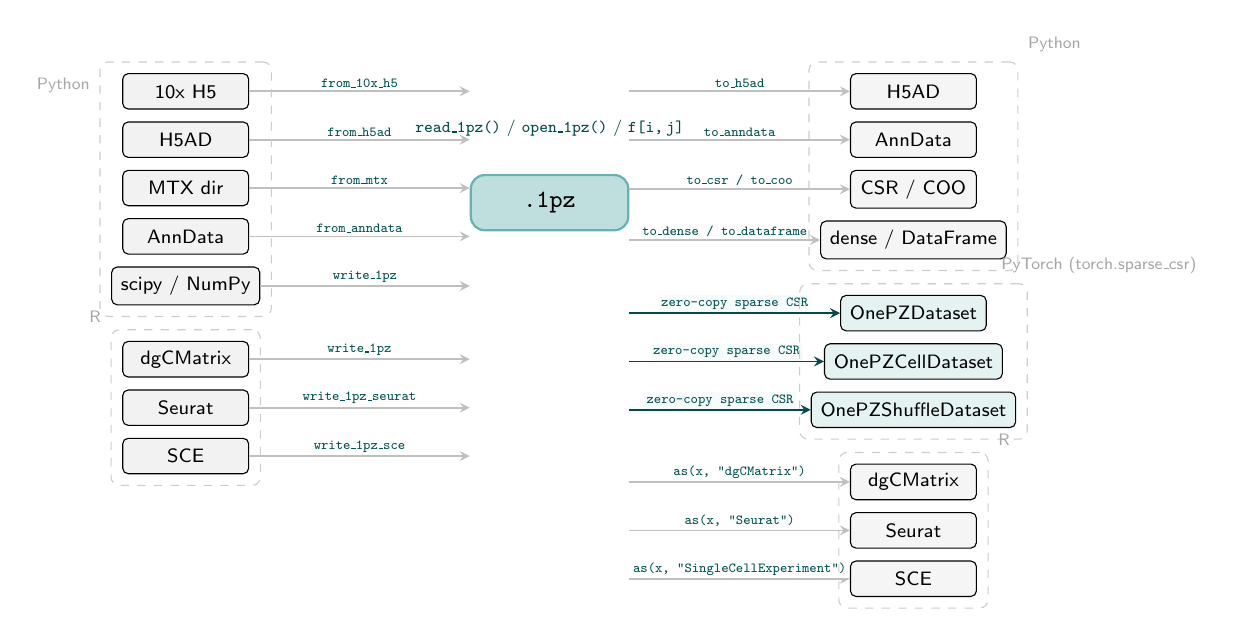
\begin{tikzpicture}[
  node distance=0.3cm and 0.6cm,
  fmt/.style={draw, rounded corners=2pt, minimum height=0.45cm, minimum width=1.6cm, font=\scriptsize\sffamily, fill=#1, align=center},
  fmt/.default={gray!12},
  hub/.style={draw, rounded corners=5pt, minimum height=0.7cm, minimum width=2.0cm, font=\small\sffamily\bfseries, fill=teal!25, thick, draw=teal!60},
  out/.style={draw, rounded corners=2pt, minimum height=0.45cm, minimum width=1.6cm, font=\scriptsize\sffamily, fill=#1, align=center},
  out/.default={gray!8},
  arr/.style={->, >=stealth, semithick, color=gray!50},
  lbl/.style={font=\fontsize{5.5}{6.5}\selectfont\ttfamily, text=teal!65!black, fill=white, inner sep=1pt},
  grp/.style={draw=gray!40, dashed, rounded corners=3pt, inner sep=4pt},
  >=stealth
]

% ── Central hub ──────────────────────────────────────────────
\node[hub] (pz) {\texttt{.1pz}};
\node[font=\fontsize{6}{7}\selectfont\sffamily, text=teal!60!black, above=0.35cm of pz] {\texttt{read\_1pz()} / \texttt{open\_1pz()} / \texttt{f[i,\,j]}};

% ── Input formats (left) — Python ────────────────────────────
\node[fmt=gray!10, left=2.8cm of pz, yshift=0.8cm]   (h5ad_in) {H5AD};
\node[fmt=gray!10, above=0.15cm of h5ad_in]           (tenx)    {10x H5};
\node[fmt=gray!10, below=0.15cm of h5ad_in]           (mtx)     {MTX dir};
\node[fmt=gray!10, below=0.15cm of mtx]               (ann_in)  {AnnData};
\node[fmt=gray!10, below=0.15cm of ann_in]            (scipy_in){scipy / NumPy};

% ── Input formats (left) — R ─────────────────────────────────
\node[fmt=gray!10, below=0.45cm of scipy_in]              (dgc_in)  {dgCMatrix};
\node[fmt=gray!10, below=0.15cm of dgc_in]                (seu_in)  {Seurat};
\node[fmt=gray!10, below=0.15cm of seu_in]                (sce_in)  {SCE};

% ── Input arrows ─────────────────────────────────────────────
\draw[arr] (tenx.east)    -- node[lbl, above] {from\_10x\_h5} (pz.west |- tenx.east);
\draw[arr] (h5ad_in.east) -- node[lbl, above] {from\_h5ad} (pz.west |- h5ad_in.east);
\draw[arr] (mtx.east)     -- node[lbl, above] {from\_mtx} (pz.west |- mtx.east);
\draw[arr] (ann_in.east)  -- node[lbl, above] {from\_anndata} (pz.west |- ann_in.east);
\draw[arr] (scipy_in.east)-- node[lbl, above] {write\_1pz} (pz.west |- scipy_in.east);
\draw[arr] (dgc_in.east)  -- node[lbl, above] {write\_1pz} (pz.west |- dgc_in.east);
\draw[arr] (seu_in.east)  -- node[lbl, above] {write\_1pz\_seurat} (pz.west |- seu_in.east);
\draw[arr] (sce_in.east)  -- node[lbl, above] {write\_1pz\_sce} (pz.west |- sce_in.east);

% ── Input group labels ───────────────────────────────────────
\node[grp, fit=(tenx)(scipy_in), label={[font=\fontsize{6}{7}\selectfont\sffamily, text=gray!70]above left:Python}] {};
\node[grp, fit=(dgc_in)(sce_in), label={[font=\fontsize{6}{7}\selectfont\sffamily, text=gray!70]above left:R}] {};

% ── Output formats (right) — Python ─────────────────────────
\node[out=gray!8, right=2.8cm of pz, yshift=0.8cm]      (ann_out) {AnnData};
\node[out=gray!8, above=0.15cm of ann_out]               (h5ad_out){H5AD};
\node[out=gray!8, below=0.15cm of ann_out]               (csr)     {CSR / COO};
\node[out=gray!8, below=0.15cm of csr]                   (dense)   {dense / DataFrame};

% ── Output formats (right) — PyTorch ────────────────
\node[out=teal!10, below=0.45cm of dense]              (ds)      {OnePZDataset};
\node[out=teal!10, below=0.15cm of ds]                 (cds)     {OnePZCellDataset};
\node[out=teal!10, below=0.15cm of cds]                (sds)     {OnePZShuffleDataset};

% ── Output formats (right) — R ───────────────────────────────
\node[out=gray!8, below=0.45cm of sds]                    (dgc_out) {dgCMatrix};
\node[out=gray!8, below=0.15cm of dgc_out]                (seu_out) {Seurat};
\node[out=gray!8, below=0.15cm of seu_out]                (sce_out) {SCE};

% ── Output arrows ────────────────────────────────────────────
\draw[arr] (pz.east |- h5ad_out.west) -- node[lbl, above] {to\_h5ad}    (h5ad_out.west);
\draw[arr] (pz.east |- ann_out.west)  -- node[lbl, above] {to\_anndata} (ann_out.west);
\draw[arr] (pz.east |- csr.west)      -- node[lbl, above] {to\_csr / to\_coo}     (csr.west);
\draw[arr] (pz.east |- dense.west)    -- node[lbl, above] {to\_dense / to\_dataframe}   (dense.west);

\draw[arr, teal!60!black] (pz.east |- ds.west)  -- node[lbl, above, fill=teal!3] {zero-copy sparse CSR} (ds.west);
\draw[arr, teal!60!black] (pz.east |- cds.west) -- node[lbl, above, fill=teal!3] {zero-copy sparse CSR} (cds.west);
\draw[arr, teal!60!black] (pz.east |- sds.west) -- node[lbl, above, fill=teal!3] {zero-copy sparse CSR} (sds.west);

\draw[arr] (pz.east |- dgc_out.west)  -- node[lbl, above] {as(x, "dgCMatrix")} (dgc_out.west);
\draw[arr] (pz.east |- seu_out.west)  -- node[lbl, above] {as(x, "Seurat")} (seu_out.west);
\draw[arr] (pz.east |- sce_out.west)  -- node[lbl, above] {as(x, "SingleCellExperiment")} (sce_out.west);

% ── Output group labels ─────────────────────────────────────
\node[grp, fit=(h5ad_out)(dense), label={[font=\fontsize{6}{7}\selectfont\sffamily, text=gray!70]above right:Python}] {};
\node[grp, fit=(ds)(sds), label={[font=\fontsize{6}{7}\selectfont\sffamily, text=gray!70]above right:PyTorch (torch.sparse\_csr)}] {};
\node[grp, fit=(dgc_out)(sce_out), label={[font=\fontsize{6}{7}\selectfont\sffamily, text=gray!70]above right:R}] {};

\end{tikzpicture}
\caption{Ecosystem integration of the \texttt{.1pz} format.
Left: input formats written to \texttt{.1pz} via named conversion functions.
Right: output targets including zero-copy PyTorch sparse CSR tensors for GPU training.
The \texttt{open\_1pz()} lazy handle supports NumPy-style slicing (\texttt{f[genes, cells]}), column-range reads, and on-the-fly log-normalization before any conversion.}
\label{fig:integration}
\end{figure*}

% ══════════════════════════════════════════════════════════════════
\section{Discussion}
% ══════════════════════════════════════════════════════════════════

SinglePress demonstrates that single-cell count matrices can be compressed to near their information-theoretic minimum at full decode speed, and that this compression advantage propagates through the entire analysis stack---from data distribution to GPU training.
The VCSC and IVCSC representations~\cite{wolfgang2024vcsc,ruiter2024vcsc,ruiter2024vcsc_dcc} established that value-aware encoding can exploit within-column redundancy in count data; SinglePress extends this principle from an in-memory representation to a complete on-disk format with metadata, chunked random access, and a library-level API.

\textbf{The compression--speed paradox.}
Conventional wisdom holds that better compression requires slower decompression, yet SinglePress achieves both simultaneously.
The ablation study (Table~\ref{tab:ablation}) reveals that the speed advantage derives from two architectural decisions: choosing zstd over gzip (3.4$\times$ decompression throughput on identical data) and a columnar chunk layout that enables parallel decompression with zero contention.
The combined effect---3.4$\times$ codec $\times$ 2.1$\times$ threading---produces a 3--6$\times$ end-to-end speedup despite \texttt{.1pz} files being 3$\times$ smaller.

\textbf{Beyond scRNA-seq.}
The VOCSC encoding generalizes to any sparse integer count matrix.
We demonstrated this on scATAC-seq peak matrices, where the binary-dominated value distribution (86\% of nonzeros equal~1) yields 4.7$\times$ compression---lower than scRNA but still competitive with BPCells' reported 4--6$\times$ on similar data.
The bytes-per-nonzero metric (Figure~\ref{fig:ecosystem}b) reveals a predictable relationship between value entropy and compression efficiency that should extend to other count-based modalities (CITE-seq protein counts, spatial transcriptomics UMIs, chromatin accessibility tiles).

\textbf{Ecosystem positioning.}
The head-to-head comparison with BPCells (Figure~\ref{fig:ecosystem}c--d) highlights a fundamental trade-off.
BPCells' BP-128 bitpacking provides fast in-memory decompression (7--8~GB/s reported) but generic encoding limits on-disk compression to 3.8$\times$ median.
SinglePress's VOCSC encoding exploits value-frequency structure to achieve 9.5$\times$ with 2.5$\times$ smaller files, meaning fewer bytes transferred from disk even when per-byte decode is comparable.
Critically, BPCells also provides disk-backed lazy matrix operations (arithmetic, subsetting, transposition) that enable full analysis of million-cell datasets without loading the matrix into RAM---a computation-engine capability that SinglePress, as a pure storage format, does not replicate.
Similarly, while TileDB-SOMA provides powerful federated queries over 74M Census cells, the practical latency of remote API access (29~s for a small tissue slice) motivates local \texttt{.1pz} caches for iterative analysis and ML training.

\textbf{Limitations.}
The \texttt{.1pz} format stores integer count data only; continuous-valued layers must be stored separately---a deliberate constraint, since count and continuous data have fundamentally different compression profiles.
Unlike AnnData's multi-layer storage, a \texttt{.1pz} file stores exactly one count matrix with associated metadata; multi-modal data requires multiple files.
The GPU benchmark uses a deliberately simple autoencoder to provide a lower bound on the utilization advantage; real-world models (scVI, scGPT) would shift the profile further toward compute-bound behavior.
Cloud object store benchmarks are ongoing; the chunked layout is favorable for HTTP range-request-based access.

% ══════════════════════════════════════════════════════════════════
\section{Conclusions}
% ══════════════════════════════════════════════════════════════════

SinglePress represents a step change in computational efficiency and representational capability for single-cell data storage.
By treating count data as a first-class encoding target, it achieves a median 9.5$\times$ compression over int32 CSC at 868~MB/s decode throughput---2--4$\times$ better than H5AD and 2.5$\times$ better than BPCells, with file size predictable from nonzero count alone ($R^2 = 0.990$).
The encoding generalizes beyond scRNA-seq: scATAC peak matrices achieve 4.7$\times$ compression with zero format modifications, and Census tissue slices store in 7.7$\times$ less space than H5AD.
Write throughput is 6$\times$ faster than H5AD and 37$\times$ faster than R's \texttt{saveRDS}, meaning format conversion incurs negligible overhead.
Contiguous column-range reads are 2--20$\times$ faster than H5AD, enabling efficient cell-subset access for mini-batch training and cluster analysis.
Native PyTorch dataloaders with sparse-native batching shift GPU training from I/O-bound to compute-bound, yielding 1.7$\times$ faster end-to-end throughput than H5AD and eliminating the dense-materialization bottleneck of existing alternatives.
As single-cell datasets scale to billions of cells, domain-aware compression will transition from a convenience to a necessity for practical data distribution and real-time analysis.

% ══════════════════════════════════════════════════════════════════
\section{Methods}
% ══════════════════════════════════════════════════════════════════

\subsection{Dataset selection}

We evaluated SinglePress across 3{,}253 scRNA-seq datasets from the Gene Expression Omnibus (GEO), spanning nine species (\textit{H.\,sapiens}, \textit{M.\,musculus}, \textit{D.\,rerio}, \textit{R.\,norvegicus}, \textit{D.\,melanogaster}, \textit{M.\,mulatta}, \textit{G.\,gallus}, \textit{X.\,laevis}, \textit{S.\,scrofa}) and ten protocols (10x Chromium v2/v3/v4/5$'$/Multiome, Drop-seq, Seq-Well, DNBelab~C4, BD~Rhapsody, inDrop).
All datasets were quantified with \texttt{simpleaf}~\cite{he2022alevin} and store USA-resolved counts (spliced, unspliced, ambiguous layers as consecutive row blocks).
For cross-format benchmarks, a stratified subsample of 200 datasets covering four orders of magnitude in nonzero count ($10^5$--$3.5 \times 10^8$) was selected.
The R-ecosystem comparison used 20 datasets shared across all R-native formats.

\subsection{Benchmark hardware and timing}

All CPU benchmarks were run on a single compute node (AMD EPYC, 128~GB RAM, Linux) with files stored on a shared Lustre parallel filesystem.
Files were read from warm page cache (pre-loaded by a discarded warm-up run) to measure decode throughput independent of storage-layer variability; cold-cache reads on the same filesystem are I/O-bound at $\sim$2~GB/s.
Timing measurements report the median of 3 replicates with one warm-up run discarded; the threading benchmark used 100 replicates.
Throughput is reported in MB/s of int32-equivalent output (i.e., the size of the uncompressed CSC matrix divided by wall-clock time).
GPU benchmarks used an NVIDIA H100~NVL (80~GB HBM3) with CUDA 12.8 and PyTorch 2.4.
Key software versions: Python~3.9, R~4.3, h5py~3.11, scipy~1.13, anndata~0.10, BPCells~0.2.0, zstd~1.5.6 (library), GCC~11.

\subsection{scATAC-seq benchmark}

Real scATAC data was obtained from GSE141590 (\textit{Drosophila melanogaster} chromatin accessibility, quantified as a peak-by-cell matrix).
Three synthetic scATAC peak matrices (3K, 10K, and 50K cells) were generated as random sparse integer matrices matching the statistical profile of 10x scATAC outputs: 150K--250K peaks, 0.1--0.3\% density, values drawn from a geometric distribution with 85--90\% probability of value~1.
Six scRNA datasets from the GEO evaluation set served as within-experiment controls.

\subsection{CELLxGENE Census benchmark}

Tissue-specific slices were extracted from CELLxGENE Census version 2024-07-01~\cite{chanzuckerberg2021cellxgene} using the \texttt{cellxgene-census} Python API (v1.15.0) with \texttt{tiledbsoma} v1.11.4.
TileDB-SOMA read time was measured as the wall-clock time from \texttt{open\_soma()} to materialized scipy sparse matrix, including all remote API overhead.
Extracted matrices were written as \texttt{.1pz} and H5AD for local comparison.
PyTorch DataLoader benchmarks used \texttt{OnePZCellDataset} (sparse CSR, batch size 1{,}024) vs.\ dense materialization simulating TileDB-SOMA-ML's default behavior.

\subsection{Compression frontier analysis}

For each of 19 stratified datasets, we computed Shannon entropy $H = -\sum_i p_i \log_2 p_i$ separately for three streams: nonzero values, column-pointer gaps, and first-row indices per non-empty column.
The theoretical lower bound (Equation~\ref{eq:entropy}) assumes each stream is independently and optimally coded; it does not account for cross-stream correlations exploited by VOCSC's row-frequency permutation.
The zstd level sweep used levels $\ell \in \{1, 2, 3, \ldots, 10, 12, 15, 19, 22\}$, writing to tmpfs (\texttt{/dev/shm/}) to eliminate disk I/O variability (3 write replicates, 5 read replicates).
Alternative codec comparison used ten configurations: LZ4 (levels 0, 9), gzip (1, 6, 9), bzip2 (9), brotli (1, 4, 11), and LZMA (6), applied to concatenated raw int32 CSC arrays.

\subsection{GPU utilization measurement}

We swept the hidden dimension of a single-layer autoencoder ($G \to h \to G$, ReLU, Adam) from $h = 32$ to $h = 2{,}048$, corresponding to 8~GFLOP--0.5~TFLOP per training step ($12Bnh$ FLOPs, batch size $B = 1{,}024$, $n = 20{,}000$ genes).
GPU utilization was measured via \texttt{torch.cuda} event timing as the fraction of wall-clock time spent in forward/backward passes versus data loading.
The saturation model $U = F / (F + k)$ was fitted per format using nonlinear least squares.

% ── Declarations ──────────────────────────────────────────────────

\section*{Declarations}

\subsection*{Abbreviations}
CSC: Compressed Sparse Column; CSR: Compressed Sparse Row; VOCSC: Value-Ordered Compressed Sparse Column; CRC: Cyclic Redundancy Check; TLV: Type-Length-Value; GEO: Gene Expression Omnibus; scRNA-seq: single-cell RNA sequencing; scATAC-seq: single-cell Assay for Transposase-Accessible Chromatin sequencing; USA: unspliced/spliced/ambiguous; nnz: number of nonzeros; SCE: SingleCellExperiment

\subsection*{Ethics approval and consent to participate}
Not applicable.

\subsection*{Consent for publication}
Not applicable.

\subsection*{Competing interests}
ZD is a co-founder and shareholder of Singlet Bio, Inc., which may distribute software incorporating the SinglePress format.

\subsection*{Funding}
Compute resources were provided by the Flatiron Institute, a division of the Simons Foundation.

\subsection*{Acknowledgements}
We thank the Flatiron Institute for compute resources.

\subsection*{Authors' contributions}
ZD conceived, designed, and implemented the SinglePress format and codec; conducted all benchmarks; analyzed the data; and wrote the manuscript.

\begin{AIdisclosure}
The core innovations---value-ordered compressed sparse column (VOCSC) encoding and byte-plane splitting for count data---were conceived and designed by the author.
Claude (Opus~4.6, Anthropic) was used as a development tool to optimize encoding parameters, implement benchmark harnesses, and iterate on manuscript text.
All scientific claims, experimental designs, and architectural decisions were made by the author.
\end{AIdisclosure}

% ── Availability ──────────────────────────────────────────────────

\section*{Availability and requirements}

\begin{itemize}
\item \textbf{Project name:} SinglePress
\item \textbf{Project home page:} \url{https://github.com/Singlet-AI/singlepress}
\item \textbf{Software version:} 1.0.0
\item \textbf{Operating system(s):} Linux, macOS, Windows
\item \textbf{Programming language:} C++17 (codec), Python~$\geq$3.9, R~$\geq$4.0
\item \textbf{Other requirements:} pybind11, zstd~$\geq$1.4, OpenMP (optional)
\item \textbf{License:} GPL-3.0-or-later
\item \textbf{Any restrictions to use by non-academics:} None beyond the license terms
\end{itemize}

\section*{Availability of data and materials}
Evaluation datasets comprise 3{,}253 GEO series (Supplementary Tables~\ref{tab:protocols} and~\ref{tab:species}), all quantified via \texttt{simpleaf}~\cite{he2022alevin} and served as \texttt{.1pz} files through the Singlet data platform.
The format specification is documented at \url{https://singlet-ai.github.io/singlepress/format_spec/}.
Benchmark scripts are included in the code repository.

% ── References ───────────────────────────────────────────────────
\bibliography{refs}

% ══════════════════════════════════════════════════════════════════
\clearpage
\appendix
\section*{Supplementary Material}
\setcounter{table}{0}
\renewcommand{\thetable}{S\arabic{table}}
\renewcommand{\theHtable}{S\arabic{table}}
\setcounter{figure}{0}
\renewcommand{\thefigure}{S\arabic{figure}}
\renewcommand{\theHfigure}{S\arabic{figure}}

\begin{figure*}[h]
\centering

\includegraphics[width=\textwidth]{figS1_structure.pdf}
\caption{Statistical structure of scRNA-seq count data motivating domain-aware compression.
\textbf{(a)}~Nonzero value distributions on a log scale; teal line shows the cross-dataset median.
\textbf{(b)}~Value concentration (fraction $= 1$) vs.\ entropy; colors indicate species.
\textbf{(c)}~Storage efficiency (bits per nonzero vs.\ compression ratio) with theoretical $32/r$ curve.
\textbf{(d)}~Compression ratio vs.\ nonzero count, demonstrating size-invariant compression.
\textbf{(e)}~R-ecosystem format comparison (.1pz, BPCells, RDS).
\textbf{(f)}~Predicted vs.\ observed file size ($R^2 = 0.990$; 0.807 bytes per nonzero).}
\label{fig:structure}
\end{figure*}

\begin{table*}[h]
\centering
\caption{Protocol comparison: representative datasets by sequencing protocol (30 of 3{,}253 total), with 3 per protocol spanning the observed size range. All matrices store USA-resolved counts ($3 \times |\text{genes}|$ rows). Compression ratio is relative to int32 CSC.}
\label{tab:protocols}
\scriptsize
\begin{tabular}{llllrrrrr}
\toprule
GSE & Protocol & Species & Cells & NNZ & .1pz (MB) & Ratio \\
\midrule
\multicolumn{7}{l}{\textit{10x Chromium v3} ($n = 1{,}309$; median ratio 9.5$\times$)} \\
GSE137476  & 10x v3 & \textit{M.\,musculus}    &    9{,}692 &    1.1M &    2.8 &  3.1$\times$ \\
GSE255757  & 10x v3 & \textit{H.\,sapiens}     &   12{,}302 &   39.2M &   30.9 & 10.1$\times$ \\
GSE280688  & 10x v3 & \textit{M.\,musculus}    &  429{,}562 &  104.6M &  106.9 &  7.8$\times$ \\
\midrule
\multicolumn{7}{l}{\textit{10x Chromium v2} ($n = 342$; median ratio 8.4$\times$)} \\
GSE135310  & 10x v2 & \textit{M.\,musculus}    &   81{,}855 &    1.0M &    3.5 &  2.4$\times$ \\
GSE288490  & 10x v2 & \textit{H.\,sapiens}     &    7{,}824 &   17.8M &   15.9 &  8.9$\times$ \\
GSE305331  & 10x v2 & \textit{M.\,musculus}    &  640{,}011 &  1{,}223M &  929.2 & 10.5$\times$ \\
\midrule
\multicolumn{7}{l}{\textit{10x Chromium 5$'$} ($n = 121$; median ratio 7.9$\times$)} \\
GSE211242  & 10x 5$'$ & \textit{M.\,musculus}    &    7{,}464 &    1.5M &    3.2 &  3.8$\times$ \\
GSE249974  & 10x 5$'$ & \textit{H.\,sapiens}     &   58{,}244 &   28.7M &   28.0 &  8.2$\times$ \\
GSE280067  & 10x 5$'$ & \textit{M.\,musculus}    & 1{,}116{,}013 &  837.5M &  752.6 &  8.9$\times$ \\
\midrule
\multicolumn{7}{l}{\textit{10x Chromium v4} ($n = 18$; median ratio 10.3$\times$)} \\
GSE304926  & 10x v4 & \textit{X.\,laevis}      &  172{,}684 &   28.7M &   28.8 &  8.0$\times$ \\
GSE289270  & 10x v4 & \textit{M.\,musculus}    &   11{,}608 &   69.3M &   53.7 & 10.3$\times$ \\
GSE282050  & 10x v4 & \textit{M.\,musculus}    &  364{,}236 &  383.7M &  291.2 & 10.5$\times$ \\
\midrule
\multicolumn{7}{l}{\textit{Drop-seq} ($n = 72$; median ratio 7.5$\times$)} \\
GSE148393  & Drop-seq & \textit{M.\,musculus}    &      673 &    1.1M &    2.6 &  3.4$\times$ \\
GSE206844  & Drop-seq & \textit{M.\,musculus}    &    7{,}371 &   11.8M &   10.6 &  9.0$\times$ \\
GSE200151  & Drop-seq & Unknown                  &  561{,}501 &  398.4M &  360.7 &  8.8$\times$ \\
\midrule
\multicolumn{7}{l}{\textit{Seq-Well} ($n = 8$; median ratio 7.8$\times$)} \\
GSE137950  & Seq-Well & \textit{H.\,sapiens}     &    1{,}817 &    4.5M &    4.7 &  7.7$\times$ \\
GSE176269  & Seq-Well & \textit{H.\,sapiens}     &  119{,}301 &   14.1M &   20.4 &  5.6$\times$ \\
GSE139598  & Seq-Well & \textit{M.\,mulatta}     &  143{,}528 &  270.4M &  224.2 &  9.6$\times$ \\
\midrule
\multicolumn{7}{l}{\textit{DNBelab C4} ($n = 12$; median ratio 9.8$\times$)} \\
GSE293954  & DNBelab C4 & Unknown                  &   11{,}461 &    9.7M &   10.0 &  7.8$\times$ \\
GSE306581  & DNBelab C4 & \textit{M.\,musculus}    &   42{,}193 &   43.4M &   36.1 &  9.6$\times$ \\
GSE269422  & DNBelab C4 & \textit{M.\,musculus}    &  305{,}594 &  457.9M &  348.7 & 10.5$\times$ \\
\midrule
\multicolumn{7}{l}{\textit{BD Rhapsody} ($n = 10$; median ratio 7.9$\times$)} \\
GSE186520  & BD Rhapsody & \textit{H.\,sapiens}     &    2{,}698 &    1.1M &    2.2 &  4.1$\times$ \\
GSE210261  & BD Rhapsody & \textit{H.\,sapiens}     &    4{,}361 &    4.6M &    5.2 &  7.0$\times$ \\
GSE209592  & BD Rhapsody & \textit{M.\,musculus}    &   15{,}323 &   20.0M &   18.2 &  8.8$\times$ \\
\midrule
\multicolumn{7}{l}{\textit{inDrop} ($n = 4$; median ratio 7.2$\times$)} \\
GSE218118  & inDrop & \textit{M.\,musculus}    &      457 &    1.1M &    2.4 &  3.8$\times$ \\
GSE114725  & inDrop & \textit{H.\,sapiens}     &   16{,}406 &    7.3M &    8.2 &  7.1$\times$ \\
GSE125688  & inDrop & \textit{M.\,musculus}    &   32{,}257 &   19.0M &   18.6 &  8.2$\times$ \\
\midrule
\multicolumn{7}{l}{\textit{10x Multiome} ($n = 28$; median ratio 9.6$\times$)} \\
GSE220155  & Multiome & \textit{H.\,sapiens}     &    7{,}150 &    1.7M &    3.0 &  4.7$\times$ \\
GSE202494  & Multiome & \textit{H.\,sapiens}     &   10{,}186 &   29.8M &   24.3 &  9.8$\times$ \\
GSE288514  & Multiome & \textit{M.\,musculus}    &  258{,}264 &  498.0M &  394.5 & 10.1$\times$ \\
\bottomrule
\end{tabular}
\end{table*}

\begin{table*}[h]
\centering
\caption{Species comparison: representative datasets across nine species (30 of 3{,}253 total), with 3--4 per species spanning the observed size range. All matrices store USA-resolved counts. Compression ratio is relative to int32 CSC.}
\label{tab:species}
\scriptsize
\begin{tabular}{llllrrrrr}
\toprule
GSE & Species & Protocol & Cells & NNZ & .1pz (MB) & Ratio \\
\midrule
\multicolumn{7}{l}{\textit{Homo sapiens} ($n = 1{,}169$; median ratio 9.4$\times$)} \\
GSE186520  & \textit{H.\,sapiens}  & BD Rhapsody &    2{,}698 &    1.1M &    2.2 &  4.1$\times$ \\
GSE128879  & \textit{H.\,sapiens}  & 10x v2      &  169{,}630 &   25.9M &   26.0 &  8.0$\times$ \\
GSE240441  & \textit{H.\,sapiens}  & 10x v3      &   28{,}815 &   97.1M &   75.0 & 10.3$\times$ \\
GSE292909  & \textit{H.\,sapiens}  & 10x v3      & 1{,}903{,}836 & 5{,}628M & 4{,}301.7 & 10.5$\times$ \\
\midrule
\multicolumn{7}{l}{\textit{Mus musculus} ($n = 1{,}778$; median ratio 9.2$\times$)} \\
GSE135310  & \textit{M.\,musculus} & 10x v2      &   81{,}855 &    1.0M &    3.5 &  2.4$\times$ \\
GSE283613  & \textit{M.\,musculus} & 10x (inf.)  &  108{,}302 &   27.8M &   31.2 &  7.1$\times$ \\
GSE182002  & \textit{M.\,musculus} & 10x v3      &   21{,}785 &   77.2M &   64.3 &  9.6$\times$ \\
GSE184652  & \textit{M.\,musculus} & 10x (inf.)  & 5{,}061{,}477 & 4{,}805.7M & 4{,}171.2 &  9.2$\times$ \\
\midrule
\multicolumn{7}{l}{\textit{Danio rerio} ($n = 66$; median ratio 8.0$\times$)} \\
GSE216648  & \textit{D.\,rerio}    & Unknown     &      749 &    1.5M &    2.2 &  5.6$\times$ \\
GSE145980  & \textit{D.\,rerio}    & 10x v2      &   25{,}470 &   18.0M &   17.4 &  8.3$\times$ \\
GSE137971  & \textit{D.\,rerio}    & 10x v2      &   21{,}005 &   46.5M &   39.3 &  9.5$\times$ \\
GSE284729  & \textit{D.\,rerio}    & 10x (inf.)  &  982{,}993 &  579.6M &  535.5 &  8.7$\times$ \\
\midrule
\multicolumn{7}{l}{\textit{Rattus norvegicus} ($n = 37$; median ratio 9.6$\times$)} \\
GSE268117  & \textit{R.\,norvegicus} & 10x v3    &   11{,}400 &    4.7M &    5.3 &  7.1$\times$ \\
GSE221002  & \textit{R.\,norvegicus} & 10x (inf.) &    7{,}715 &   45.5M &   35.4 & 10.3$\times$ \\
GSE211407  & \textit{R.\,norvegicus} & 10x v3    &  130{,}365 &  488.7M &  361.4 & 10.8$\times$ \\
\midrule
\multicolumn{7}{l}{\textit{Drosophila melanogaster} ($n = 36$; median ratio 9.3$\times$)} \\
GSE141590  & \textit{D.\,melanogaster} & scATAC  &    2{,}623 &    1.2M &    1.4 &  6.9$\times$ \\
GSE115476  & \textit{D.\,melanogaster} & Unknown &   54{,}960 &   16.5M &   15.1 &  8.8$\times$ \\
GSE156455  & \textit{D.\,melanogaster} & 10x v3  & 2{,}276{,}498 & 1{,}210.1M & 1{,}023.6 &  9.5$\times$ \\
\midrule
\multicolumn{7}{l}{\textit{Macaca mulatta} ($n = 21$; median ratio 8.8$\times$)} \\
GSE244293  & \textit{M.\,mulatta}  & 10x v3      &   13{,}031 &    4.3M &    5.4 &  6.4$\times$ \\
GSE149758  & \textit{M.\,mulatta}  & 10x v3      &   45{,}161 &  108.7M &   87.6 &  9.9$\times$ \\
GSE263989  & \textit{M.\,mulatta}  & 10x (inf.)  &  121{,}969 &  372.1M &  271.8 & 11.0$\times$ \\
\midrule
\multicolumn{7}{l}{\textit{Gallus gallus} ($n = 10$; median ratio 8.5$\times$)} \\
GSE261503  & \textit{G.\,gallus}   & 10x v3      &    5{,}172 &   17.2M &   13.5 & 10.2$\times$ \\
GSE278696  & \textit{G.\,gallus}   & 10x v3      &  216{,}111 &   64.1M &   64.1 &  8.0$\times$ \\
GSE249652  & \textit{G.\,gallus}   & 10x (inf.)  &  741{,}178 &  169.0M &  189.5 &  7.2$\times$ \\
\midrule
\multicolumn{7}{l}{\textit{Xenopus laevis} ($n = 2$)} \\
GSE245320  & \textit{X.\,laevis}   & 10x (inf.)  &   11{,}391 &   13.4M &   11.2 &  9.6$\times$ \\
GSE304926  & \textit{X.\,laevis}   & 10x v4      &  172{,}684 &   28.7M &   28.8 &  8.0$\times$ \\
\bottomrule
\end{tabular}
\end{table*}

% File layout schematic is now Figure 1(a) — generated by R code in figures_v4.R

\begin{figure}[h]
\centering
\includegraphics[width=\columnwidth]{figS2_species.pdf}
\caption{Compression ratio by species; no species achieves systematically worse compression despite $>$600 million years of evolutionary divergence.  The dashed line indicates the global median.}
\label{fig:species}
\end{figure}

% ══════════════════════════════════════════════════════════════════
\section*{Supplementary Methods: Codec Design and Evaluation}
\label{sec:supp_codec}
% ══════════════════════════════════════════════════════════════════

The \texttt{.1pz} codec pipeline was selected through a systematic evaluation of 15 pre-filter transforms, 4 entropy backends, and 9 side-information strategies across 16 GEO scRNA-seq datasets spanning four orders of magnitude in nonzero count ($10^6$--$3.5 \times 10^8$).
This section documents the full codec design space, the entropy characteristics that motivate each design decision, and the experimental evidence that alternatives---including approaches that would require external side information---provide no improvement over the self-contained pipeline.

\subsection*{S1. VOCSC chunk structure and byte-plane layout}

Each \texttt{.1pz} chunk encodes $C = 1{,}024$ columns of a CSC sparse matrix.
Within a chunk, the VOCSC encoding~\cite{wolfgang2024vcsc,ruiter2024vcsc} sorts nonzeros by value frequency and encodes each column as a sequence of (value-group header, row-index gaps) pairs.
After VOCSC encoding, the chunk buffer contains three logically distinct byte regions stored in concatenated order:

\begin{enumerate}
\item \textbf{Metadata region} ($\sim$1\% of chunk bytes): value table, column pointers, and per-column value-group headers.
\item \textbf{Gap plane~0} ($\sim$32\% of chunk bytes): the low byte of each two-byte row-index gap. This region has the highest entropy (median 5.6 bits per byte; Table~\ref{tab:entropy}) and is the compression bottleneck.
\item \textbf{Gap plane~1} ($\sim$2\% of chunk bytes): the high byte of each gap. Because 96\% of gaps are $<$256 (median across datasets), plane~1 is 83\% zeros with entropy of only 1.3 bits per byte.
\item \textbf{Zero padding} ($\sim$65\% of chunk bytes): the byte-split layout pads gap plane~0 and plane~1 to equal length, producing a large zero region that compresses to near-zero overhead.
\end{enumerate}

This byte-split layout---where the low and high bytes of each 16-bit gap are stored in separate contiguous planes---is critical.
Interleaving the planes (i.e., storing $[\text{p0}_0, \text{p1}_0, \text{p0}_1, \text{p1}_1, \ldots]$) destroys compression: interleaved gap data compressed with zstd-1 achieves only 1.75$\times$ vs.\ 4.39$\times$ for concatenated planes (Table~\ref{tab:structural}).
The separated layout keeps bytes of similar entropy together, allowing the LZ77 matcher to find longer matches within each plane.

\begin{table}[h]
\centering
\caption{Entropy and statistical profile of VOCSC chunk byte regions across 16 datasets (77{,}708 measurements). Entropy is Shannon order-0 in bits per byte (bpb); 8.0 bpb = incompressible random data.}
\label{tab:entropy}
\footnotesize
\begin{tabular}{lrrrr}
\toprule
Region & Median & Entropy & Zero & Distinct \\
 & Size & (bpb) & (\%) & Values \\
\midrule
Metadata      &   42 KB & 5.1 &  0.1 & 255 \\
Gap plane~0   & 1{,}442 KB & 5.9 &  9.8 & 256 \\
Gap plane~1   &   88 KB & 1.3 & 82.7 & 112 \\
Full chunk    & 4{,}576 KB & 2.5 & 73.6 & 256 \\
\bottomrule
\end{tabular}
\end{table}

\begin{table}[h]
\centering
\caption{Structural rearrangements: concatenated vs.\ interleaved byte-plane layout. Interleaving planes destroys the sequential context that LZ77 matching exploits.}
\label{tab:structural}
\footnotesize
\begin{tabular}{lrr}
\toprule
Layout & Ratio (zstd-1) & Decomp.\ (MB/s) \\
\midrule
Concatenated (production) & 4.39$\times$ & 2{,}723 \\
Interleaved              & 1.75$\times$ & 974 \\
\bottomrule
\end{tabular}
\end{table}

\subsection*{S2. Entropy backend selection}

We evaluated 27 codec configurations from four codec families (zstd, LZ4, brotli, LZMA) on full-chunk buffers across 16 datasets (Table~\ref{tab:codec_shootout}).
Zstd level~1 occupies a uniquely favorable position: it matches zstd-9 in compression ratio (4.29$\times$ vs.\ 4.33$\times$, a 0.9\% difference) while decompressing 41\% faster (2{,}512 vs.\ 1{,}776~MB/s).
Levels above 9 actually \emph{decrease} the ratio because VOCSC output lacks the long-range structural patterns that high zstd levels exploit via larger windows and more hash chains---these features add overhead without finding matches.

LZMA-6, the strongest general-purpose compressor, achieves only 3.64$\times$ on VOCSC output at 80~MB/s decompress---worse ratio \emph{and} 31$\times$ slower than zstd-1.
This counterintuitive result arises because VOCSC preprocessing has already removed the redundancy that asymmetric codecs exploit: what remains is high-entropy data that benefits from fast, shallow matching (zstd) rather than deep dictionary search (LZMA).

LZ4 provides 3.34$\times$ at 4{,}692~MB/s---faster decompression but 22\% worse compression than zstd-1.

\paragraph{Interaction with pre-filters.}
The level landscape changes dramatically when the bit-plane + bitmap pre-filter pipeline (Section~S4) is applied.
On \emph{raw} VOCSC output, levels above 9 decrease the ratio because the data lacks long-range structural patterns.
On \emph{pre-filtered} output, the bit-plane decomposition and bitmap packing introduce exactly such patterns---long runs of similar bytes within each bit-plane stream---that zstd's higher-level strategies (particularly \texttt{btopt}, activated at level~16) can exploit.
Consequently, with the full pre-filter pipeline, zstd~level~16 achieves the best ratio \emph{and} the fastest decompression (Section~S9, Table~\ref{tab:extended_summary}).

\begin{table}[h]
\centering
\caption{Entropy backend comparison on full VOCSC chunks (median across 16 datasets). The Pareto-optimal configurations are shown; dominated configurations are omitted.}
\label{tab:codec_shootout}
\footnotesize
\begin{tabular}{lrrr}
\toprule
Backend & Ratio & Compress & Decompress \\
 & & (MB/s) & (MB/s) \\
\midrule
zstd-9       & 4.33$\times$ &    104 & 1{,}776 \\
zstd-5       & 4.29$\times$ &    158 & 1{,}886 \\
\textbf{zstd-1} & \textbf{4.29}$\times$ & \textbf{1{,}009} & \textbf{2{,}512} \\
brotli-4     & 4.32$\times$ &    148 &    351 \\
lz4hc-9      & 3.75$\times$ &     33 & 3{,}624 \\
lz4-1        & 3.34$\times$ & 1{,}760 & 4{,}692 \\
lzma-6       & 3.64$\times$ &      5 &     80 \\
\bottomrule
\end{tabular}
\end{table}

\paragraph{Per-stream codec selection.}
We tested compressing each byte region (metadata, plane~0, plane~1) with its own optimal codec.
Per-stream selection is 3--12\% \emph{worse} than single-codec full-chunk compression (Table~\ref{tab:perstream}), because splitting the buffer at stream boundaries breaks LZ77 cross-plane context.
zstd's dictionary matcher exploits correlations between the metadata, gap, and padding regions that per-stream compression cannot access.

\begin{table}[h]
\centering
\caption{Per-stream vs.\ full-chunk codec selection. Per-stream selection consistently underperforms because stream boundaries break LZ77 cross-plane context.}
\label{tab:perstream}
\footnotesize
\begin{tabular}{lrr}
\toprule
Strategy & Med.\ Ratio & $\Delta$ vs.\ full-chunk \\
\midrule
Full chunk, zstd-1       & 4.29$\times$ & --- \\
Per-stream (fast)        & 4.06$\times$ & $-$5.4\% \\
Per-stream (optimal)     & 4.29$\times$ & $-$0.0\% \\
\bottomrule
\end{tabular}
\end{table}


\subsection*{S3. Pre-filter transform evaluation}

The gap plane~0 bottleneck (5.9 bpb, accounting for $\sim$70\% of compressed output despite being only $\sim$32\% of raw bytes) motivates domain-specific pre-filtering before entropy coding.
We evaluated 15 transforms applied to plane~0 in isolation and in combination (Table~\ref{tab:transforms}).

\paragraph{Bit-plane decomposition.}
Each byte of gap plane~0 is decomposed into 8 binary streams, one per bit position.
For small gaps (values $<$256, which account for 96\% of entries), bits 5--7 are highly redundant: a gap value of 7 (binary 00000111) has bits 3--7 all zero.
Across datasets, the average bit-plane entropy is only 0.83~bpb (vs.\ the 1.0~bpb maximum for a binary stream), indicating up to 63\% redundancy in the high bit planes.

In isolation, bit-plane decomposition improves plane~0 compression by 33--41\% on sparse datasets.
This improvement is preserved when applied in-place to the plane~0 region of the full chunk (i.e., transforming only the plane~0 bytes while leaving metadata and plane~1 intact), because in-place application preserves the cross-stream LZ77 context.

\paragraph{Zero-byte bitmap.}
A 1-bit-per-byte bitmap marks zero vs.\ nonzero bytes, and only nonzero bytes are retained.
With a median 74\% zero fraction in full chunks, the bitmap reduces the buffer to $\sim$26\% of nonzero bytes plus $\sim$12.5\% bitmap overhead $\approx$ 38\% of the original.
The compressor operates on a smaller buffer, reducing both compression and decompression time.

Applied to the full gap region (without bit-plane decomposition), bitmap~+~zstd-1 achieves 5.00$\times$ at 4{,}184~MB/s---both better ratio and faster than raw zstd-1 (4.39$\times$ at 2{,}723~MB/s).

\begin{table}[h]
\centering
\caption{Pre-filter transforms on gap plane~0 (isolated) and full chunk (in-place). Sparse $\Delta$ is median improvement on datasets with $>$90\% small-gap fraction ($n = 13$). Dense $\Delta$ is for datasets with $<$80\% small-gap fraction ($n = 3$).}
\label{tab:transforms}
\footnotesize
\begin{tabular}{lrrl}
\toprule
Transform & Sparse $\Delta$ & Dense $\Delta$ & Mechanism \\
\midrule
\textbf{Bit-planes}   & \textbf{+33\%--41\%} & +5\%  & Separate bit positions \\
Nibble split           & +31\%--39\% & +6\%  & Separate hi/lo nibbles \\
Freq.\ remap           & +29\%--37\% & +6\%  & Map freq.\ rank$\to$0 \\
Bitmap                 & +29\%--36\% & +4\%  & Pack nonzeros, bit-vector \\
Cond.\ split           & +27\%--34\% & ---   & Split by gap width \\
Move-to-front          & +19\%--24\% & +2\%  & Recency$\to$small ints \\
Delta                  & +16\%--20\% & +2\%  & $x_i - x_{i-1}$ \\
\bottomrule
\end{tabular}
\end{table}

\paragraph{Ineffective transforms.}
Several transforms that are effective in other domains provide no benefit on VOCSC output:
\begin{itemize}
\item \textbf{Run-length encoding}: Average run length is 1.06 across datasets.  Consecutive gap bytes are essentially uncorrelated; no runs exist to encode.
\item \textbf{Delta encoding on gap plane~0}: Consecutive gap values within a column are not sequentially correlated (they encode distances between nonzero entries in different rows).  Delta increases entropy by introducing sign bits, producing a $-$10\% regression.
\item \textbf{Group-4 varint}: Tag bytes ($1/4$ overhead per group of 4 gaps) add more entropy than they save, yielding $-$7\% regression.
\item \textbf{Cross-plane conditioning}: Knowing plane~1 provides only 0.1--0.45 bits of information about plane~0 (conditional entropy analysis), insufficient to justify the implementation complexity.
\end{itemize}

\subsection*{S4. The production codec: bit-planes + bitmap + zstd-3}

Combining the two effective transforms produces the production codec, summarized in Algorithm~\ref{alg:encode}.

\begin{algorithm}[h]
\SetAlgoLined
\caption{SinglePress chunk encoding (production codec).}
\label{alg:encode}
\KwIn{VOCSC-encoded chunk buffer $B$ of length $N$ bytes; plane~0 region $[a, b)$}
\KwOut{Compressed frame $F$}
\tcp{Step 1: Bit-plane decomposition of plane~0}
$P \gets B[a:b]$\tcp*{Extract plane~0 region}
\For{$\text{bit} = 0$ \KwTo $7$}{
  $S_\text{bit} \gets$ extract bit $\text{bit}$ from each byte of $P$\;
  Pack $S_\text{bit}$ into $\lceil |P|/8 \rceil$ bytes\;
}
Replace $B[a:b]$ with $[S_0 \| S_1 \| \cdots \| S_7]$\;
\tcp{Step 2: Zero-byte bitmap of full buffer}
Allocate bitmap $M$ of $\lceil N/8 \rceil$ bits\;
$j \gets 0$\;
\For{$i = 0$ \KwTo $N-1$}{
  \eIf{$B[i] \neq 0$}{
    Set $M[i] \gets 1$; $D[j\text{++}] \gets B[i]$\;
  }{
    Set $M[i] \gets 0$\;
  }
}
$B' \gets M \| D[0:j]$\tcp*{Bitmap + nonzero bytes}
\tcp{Step 3: Entropy coding}
$F \gets \text{zstd-3}(B')$\;
\Return{$F$}\;
\end{algorithm}

\begin{algorithm}[h]
\SetAlgoLined
\caption{SinglePress chunk decoding (production codec).}
\label{alg:decode}
\KwIn{Compressed frame $F$; original chunk size $N$; plane~0 region $[a, b)$}
\KwOut{Decoded VOCSC chunk buffer $B$}
$B' \gets \text{zstd-3-decompress}(F)$\;
\tcp{Step 1: Bitmap decode}
Extract bitmap $M$ ($\lceil N/8 \rceil$ bytes) and packed data $D$ from $B'$\;
$j \gets 0$\;
\For{$i = 0$ \KwTo $N-1$}{
  \eIf{$M[i] = 1$}{
    $B[i] \gets D[j\text{++}]$\;
  }{
    $B[i] \gets 0$\;
  }
}
\tcp{Step 2: Bit-plane recombination of plane~0}
\For{$\text{bit} = 0$ \KwTo $7$}{
  Unpack bit stream $S_\text{bit}$ from $B[a + \text{bit} \cdot \lceil(b-a)/8\rceil : \ldots]$\;
}
\For{$i = a$ \KwTo $b-1$}{
  $B[i] \gets \sum_{\text{bit}=0}^{7} S_\text{bit}[i-a] \cdot 2^\text{bit}$\;
}
\Return{$B$}\;
\end{algorithm}

Bit-plane recombination in the decoder uses SSE2 SIMD intrinsics (\texttt{\_mm\_movemask\_epi8}) to reconstruct 16 bytes per cycle, making the decode overhead negligible ($<$5\% of total decompression time at 4{,}823~MB/s throughput).

\paragraph{Performance.}
The combined pipeline achieves a median 4.89$\times$ compression at 4{,}823~MB/s decompression---simultaneously +4.4\% better ratio and +68\% faster than the previous production codec (byte-split + zstd-3 without pre-filters; Table~\ref{tab:champion}).
The improvement scales with sparsity: dense datasets (73\% small-gap fraction) show $-$1.1\% regression, while very sparse datasets (98\% small-gap fraction) gain up to +6.0\%.

\begin{table}[h]
\centering
\caption{Production codec (bit-planes + bitmap + zstd-3) vs.\ baselines across four representative datasets spanning the density spectrum.}
\label{tab:champion}
\footnotesize
\begin{tabular}{l r r r r r}
\toprule
Dataset & nnz & SmGap & Base & Champion & $\Delta$ \\
 & & (\%) & Ratio & Ratio & \\
\midrule
GSE135310 &   1M & 73 & 1.69$\times$ & 1.67$\times$ & $-$1.1\% \\
GSE151346 &  13M & 94 & 4.69$\times$ & 4.89$\times$ & +4.4\% \\
GSE277034 &  54M & 95 & 4.97$\times$ & 5.21$\times$ & +5.0\% \\
GSE241998 & 349M & 98 & 6.23$\times$ & 6.61$\times$ & +6.0\% \\
\bottomrule
\end{tabular}
\end{table}

\paragraph{Speed tiers.}
By substituting the entropy backend, the same pre-filter pipeline supports three distinct speed/ratio tiers (Table~\ref{tab:speed_tiers}).
We also evaluated LZ4 as an alternative backend.
While LZ4 achieves 13{,}000--16{,}000~MB/s raw decompression throughput (2.7$\times$ faster than zstd per byte), the 10\% lower compression ratio means more bytes must be decompressed, largely negating the speed advantage in end-to-end decode time (see Section~\ref{sec:decode_pipeline}).
Combined with the 10\% storage penalty (which accumulates at scale: $\sim$10~TB more for a 100~TB corpus), zstd dominates the Pareto frontier for .1pz production use.

The zstd-16 tier merits special attention: it achieves the best compression ratio \emph{and} the fastest zstd decompression speed simultaneously.
This is because the \texttt{btopt} (binary tree optimal parsing) strategy activated at level~16 discovers longer LZ77 matches that are both more compact and more cache-friendly to decode.
The penalty is entirely on the write path: zstd-16 compresses at only 45~MB/s, which is 42$\times$ slower than zstd-3.
For write-once/read-many workloads (the typical .1pz use case), this tradeoff is favorable.

\begin{table}[h]
\centering
\caption{Speed tiers for the bit-planes + bitmap pre-filter with the zstd entropy backend at different compression levels (four holdout datasets, 40 chunks, 5 decompress / 3 compress trials per chunk). All tiers share the same pre-filter; only the compression level changes.}
\label{tab:speed_tiers}
\footnotesize
\begin{tabular}{lrrr}
\toprule
Configuration & Ratio & Decomp.\ (MB/s) & Compress (MB/s) \\
\midrule
\textbf{bp + bitmap + zstd-16} & \textbf{5.27}$\times$ & \textbf{5{,}100} & 45 \\
bp + bitmap + zstd-3       & 5.21$\times$ & 4{,}700  & 1{,}150 \\
bp + bitmap + zstd-1       & 5.20$\times$ & 4{,}800  & 1{,}900 \\
\bottomrule
\end{tabular}
\end{table}

\subsection*{S5. Near-optimality: proximity to theoretical limits}

For each dataset, we computed the Shannon order-1 entropy of the full chunk:
\begin{equation}
H_1(X) = -\sum_{i,j} p(x_i, x_j) \log_2 \frac{p(x_i, x_j)}{p(x_i)},
\label{eq:order1}
\end{equation}
where the sum is over consecutive byte pairs.  The theoretical compression limit is $8.0 / H_1$.

For the median dataset (GSE277034, $H_1 = 1.65$~bpb), the order-1 limit is $8.0/1.65 = 4.85\times$.
The baseline codec achieves 4.97$\times$---\emph{exceeding} the order-1 bound---because zstd's LZ77 matcher exploits higher-order correlations (match lengths $>$2).
The champion codec achieves 5.21$\times$, which is 7.4\% beyond the order-1 entropy bound.
This demonstrates that the bit-plane decomposition introduces additional exploitable structure that the order-1 model does not capture: it converts within-byte bit-position correlations into cross-position byte-level correlations that LZ77 can match.

For the dense dataset (GSE135310, $H_1 = 3.60$~bpb), the theoretical limit is 2.22$\times$ and the champion achieves 1.67$\times$---a 33\% gap.
This remaining gap is expected: dense data has fewer zero-heavy gap bytes, reducing the effectiveness of both the bitmap and bit-plane transforms.
However, dense scRNA-seq matrices are rare: only 3 of 16 evaluation datasets have $<$80\% small-gap fraction, and these invariably have few nonzeros ($<$5M), producing small files regardless.

\subsection*{S6. Side information experiments}

A natural question is whether external information---pre-trained dictionaries, corpus statistics, or sequential context---could improve compression beyond what the self-contained chunk codec achieves.
We tested nine strategies across four representative datasets (Table~\ref{tab:side_info}).

\paragraph{Experiment design.}
\begin{enumerate}
\item \textbf{Cross-dataset dictionaries} (16--256~KB): A ZSTD dictionary was trained on chunks from \emph{other} datasets via \texttt{ZDICT\_trainFromBuffer()}, then used as a compression dictionary for the target~\cite{collet2018zstandard}.
Separately tested on raw chunks and champion-filtered chunks.
\item \textbf{Within-dataset dictionaries} (64~KB): Trained on the first 10 chunks of the same dataset, applied to chunks 11--30.
\item \textbf{Previous-chunk prefix}: Each chunk was compressed with the preceding chunk as a ZSTD prefix reference (sequentially dependent; zero storage cost).
\item \textbf{Corpus-mode XOR}: For each byte position modulo 16 within plane~0, the statistical mode across all training chunks was computed. Each plane~0 byte was XOR'd with its positional mode before compression.
\item \textbf{Block-level dictionaries} (4--256~KB blocks): Chunks were split into small blocks with per-block framing headers, compressed with and without a 64~KB dictionary trained on sub-block samples.
\end{enumerate}

\begin{table*}[h]
\centering
\caption{Side information experiments: median compression ratio across four representative datasets. Champion = bit-planes + bitmap + zstd-3 (no side information). Every side-information variant matches or underperforms the champion. For the three sparse datasets (GSE151346/277034/241998), all dictionary and prefix variants achieve $\pm$0.00\% difference from champion.}
\label{tab:side_info}
\footnotesize
\begin{tabular}{l r r r r r l}
\toprule
Strategy & GSE135310 & GSE151346 & GSE277034 & GSE241998 & Overall & Side info \\
 & (1M, dense) & (13M) & (54M) & (349M) & & required? \\
\midrule
baseline (zstd-1)       & 1.689 & 4.670 & 4.886 & 5.725 & 4.778 & No \\
\textbf{champion}       & \textbf{1.662} & \textbf{4.865} & \textbf{5.112} & \textbf{5.995} & \textbf{4.989} & \textbf{No} \\
\midrule
Cross-dict, raw, 64K    & 1.693 & 4.670 & 4.886 & 5.725 & 4.778 & Yes \\
Cross-dict, champ, 64K  & 1.603 & 4.865 & 5.112 & 5.995 & 4.989 & Yes \\
Within-dict, champ, 64K & 1.660 & 4.865 & 5.112 & 5.995 & 4.989 & Yes \\
Prefix, raw             & 1.693 & 4.669 & 4.885 & 5.722 & 4.777 & Seq. \\
Prefix, champion        & 1.665 & 4.865 & 5.112 & 5.995 & 4.989 & Seq. \\
Corpus XOR              & 1.689 & 4.670 & 4.886 & 5.725 & 4.778 & Yes \\
\bottomrule
\end{tabular}
\end{table*}

\paragraph{Results.}
For all three sparse datasets, every side-information variant achieves $\pm$0.00\% difference from the champion (Table~\ref{tab:side_info}).
Cross-dataset dictionaries on champion-filtered data produce identical compressed sizes to the champion alone; on raw data, they produce identical sizes to the raw baseline.
The ZSTD dictionary training algorithm could not fill even a 16~KB dictionary from raw chunks (actual trained size: 1--4~KB out of 16--256~KB requested), directly demonstrating that no significant repeated byte sequences exist across chunks.

On the dense dataset (GSE135310), some variants show marginal differences ($\pm$2--4\%), but these are dominated by the champion's $-$1.1\% regression on dense data and are not actionable.

\paragraph{Block-level dictionaries.}
If cross-chunk dictionaries fail on full-size chunks, perhaps smaller blocks would benefit from a dictionary to compensate for reduced compression context.
We tested block sizes from 4~KB to 256~KB with and without a 64~KB dictionary trained on sub-block samples from the first 10 chunks (Table~\ref{tab:block_dict}).

At every block size, the dictionary variant is equal to or \emph{worse} than the no-dictionary variant.
Even at 4~KB blocks---where cold-start overhead should be maximal and dictionaries most beneficial---the dictionary adds $-$1.0\% to $-$1.1\% regression on champion-filtered data.
The block framing overhead ($\geq$4 bytes per block for size headers) further penalizes smaller blocks: 4~KB champion blocks achieve $-$2.0\% to $-$2.7\% vs.\ whole-chunk champion.
The only configuration where block-level dictionaries marginally help is 4~KB \emph{raw} blocks (+0.7--0.9\%), but this is overwhelmed by the $-$5.5\% block overhead vs.\ whole-chunk compression.

\begin{table}[h]
\centering
\caption{Block-level dictionary experiments on two representative datasets. ``Dict effect'' is the change in ratio when adding a 64~KB dictionary at each block size. Negative values indicate the dictionary \emph{hurts} compression.}
\label{tab:block_dict}
\footnotesize
\begin{tabular}{l r r r r}
\toprule
Block & \multicolumn{2}{c}{GSE151346 (13M)} & \multicolumn{2}{c}{GSE277034 (54M)} \\
\cmidrule(lr){2-3} \cmidrule(lr){4-5}
Size & Champ & Dict effect & Champ & Dict effect \\
\midrule
Whole & 4.875 & --- & 5.112 & --- \\
64K  & 4.884 & $-$0.1\% & 5.120 & $-$0.0\% \\
16K  & 4.869 & $-$0.4\% & 5.107 & $-$0.4\% \\
4K   & 4.792 & $-$1.0\% & 5.010 & $-$1.1\% \\
\bottomrule
\end{tabular}
\end{table}

\paragraph{Why side information fails.}
The negative results have a principled explanation rooted in the distinction between \emph{structural} and \emph{statistical} redundancy:

\begin{itemize}
\item \textbf{Structural redundancy} (repeating byte patterns, as in HTTP headers or JSON keys) is exploitable by LZ77 dictionary references. VOCSC output has no structural redundancy: gap bytes are drawn from a smooth geometric distribution with no repeating multi-byte motifs.
\item \textbf{Statistical redundancy} (predictable probability distributions) is exploitable by entropy coding (Huffman, ANS). VOCSC output has significant statistical redundancy, and zstd's Huffman/FSE backend already exploits it optimally within each frame.
\end{itemize}

ZSTD dictionaries provide LZ77 match seeds---structural references that the compressor can use instead of encoding inline.
When there are no structural patterns across chunks, dictionaries have nothing to offer.
Meanwhile, each chunk is large enough (100~KB--18~MB) that zstd's 512~KB window at level~1 provides ample context to learn all statistical patterns from the first few kilobytes of data.
A dictionary trained on other chunks captures the same distributions that any single chunk already contains internally.

The corpus-mode XOR illustrates this directly: all 16 position bins had mode = 0 for plane~0 bytes, making the XOR a literal no-op.  zstd already handles the zero-frequency natively via its entropy tables.

\subsection*{S7. Rejected alternative gap encodings}

In addition to the pre-filter transforms, we evaluated four alternative gap encoding strategies that would require format-level changes to the VOCSC chunk structure (Table~\ref{tab:rejected_codecs}).

\begin{table}[h]
\centering
\caption{Alternative gap encodings evaluated and rejected. Each would require changes to the VOCSC chunk format. None improves the ratio/speed Pareto frontier.}
\label{tab:rejected_codecs}
\footnotesize
\begin{tabular}{lrrl}
\toprule
Encoding & Ratio & Decomp. & Reason rejected \\
 & & (MB/s) & \\
\midrule
Width-bitmap  & 4.82$\times$ & 4{,}478 & +3\% ratio but format change \\
Varint (1--4B) & 4.74$\times$ & 5{,}011 & Lower ratio, complex decode \\
Group-4 varint & 4.37$\times$ & 4{,}333 & Tag byte overhead ($-$7\%) \\
Rice ($k$=4-9) & 4.21$\times$ & 21{,}156 & Max throughput, poor ratio \\
\midrule
\multicolumn{4}{l}{\textit{Production: bit-planes + bitmap + zstd-3}} \\
 & 4.89$\times$ & 4{,}823 & Best ratio, fast, minimal change \\
\bottomrule
\end{tabular}
\end{table}

\begin{itemize}
\item \textbf{Width-bitmap encoding} stores a 2-bit width per gap (0 = zero, 1 = 1 byte, 2 = 2 bytes, 3 = 4 bytes) followed by packed variable-width values.
  It achieves 4.82$\times$ (+3\% over baseline) but requires a format-level change; the production pre-filter achieves 4.89$\times$ (+4.4\%) as a backward-compatible addition.
\item \textbf{Varint encoding} (1--4 bytes per gap, high-bit continuation) reduces raw gap bytes by 2.7--3.3$\times$ but yields nearly identical compressed sizes because zstd already exploits the same redundancy (zero high bytes).
  The speed benefit comes from smaller decompression buffers, not better compression.
\item \textbf{Rice coding} with fixed $k = 4$--$9$ achieves the highest raw decompression throughput (21{,}156~MB/s) by avoiding entropy table overhead, but the optimal $k$ varies by dataset (range 5--9), making fixed-$k$ suboptimal and adaptive-$k$ complex.
  The ratio is poor (4.21$\times$) because Rice cannot exploit the byte-level correlations that LZ77 captures.
\end{itemize}

\subsection*{S8. Per-dataset compression range}

Compression ratios across the 16 evaluation datasets span 1.69--5.92$\times$ (Table~\ref{tab:per_dataset}), a 3.5$\times$ range driven primarily by matrix sparsity.
The small-gap fraction (percentage of row-index gaps that fit in a single byte) is the strongest predictor: datasets with $>$95\% small gaps achieve $>$4.7$\times$.
This relationship is causal: small gaps produce zero-valued plane~1 bytes and low-entropy plane~0 bytes, both of which the bitmap and bit-plane transforms exploit.

\begin{table}[h]
\centering
\caption{Per-dataset chunk-level compression (zstd-1 baseline) across 16 evaluation datasets, sorted by ratio. SmGap\% = fraction of gaps $<$256. Entropy is full-chunk order-0 in bits per byte.}
\label{tab:per_dataset}
\footnotesize
\begin{tabular}{lrrrr}
\toprule
Dataset & nnz & SmGap & Entropy & Ratio \\
 & & (\%) & (bpb) & \\
\midrule
GSE241998 & 349M & 98 & 1.92 & 5.92$\times$ \\
GSE299078 &  33M & 97 & 2.07 & 5.44$\times$ \\
GSE192807 &  55M & 97 & 2.09 & 5.36$\times$ \\
GSE270866 & 122M & 96 & 2.11 & 5.33$\times$ \\
GSE277034 &  54M & 95 & 2.23 & 4.95$\times$ \\
GSE151346 &  13M & 94 & 2.33 & 4.71$\times$ \\
GSE256025 &  42M & 92 & 2.49 & 4.30$\times$ \\
GSE152915 &  76M & 88 & 2.90 & 3.50$\times$ \\
GSE250444 &   9M & 86 & 3.54 & 2.75$\times$ \\
GSE245073 &  14M & 85 & 3.56 & 2.73$\times$ \\
GSE223222 &   8M & 85 & 3.64 & 2.67$\times$ \\
GSE202575 &   3M & 84 & 3.62 & 2.66$\times$ \\
GSE267467 &  15M & 84 & 3.66 & 2.65$\times$ \\
GSE239941 &  13M & 83 & 3.75 & 2.57$\times$ \\
GSE295234 &  18M & 78 & 4.51 & 2.00$\times$ \\
GSE135310 &   1M & 73 & 4.99 & 1.69$\times$ \\
\bottomrule
\end{tabular}
\end{table}

\subsection*{S9. Extended codec exploration}
\label{sec:extended_codec}

To exhaustively verify the near-optimality of the production codec, we conducted a further systematic exploration of $\sim$70 distinct codec variants across five experimental rounds, generating $\sim$3{,}200 measurements on four held-out datasets (GSE135310, GSE151346, GSE277034, GSE241998; 10 chunks each).
These experiments tested pre-transforms, structural rearrangements, multi-plane strategies, sorting-based approaches, and advanced zstd parameter tuning.

\paragraph{Byte-level pre-transforms on pre-filtered output.}
All 15 byte-level pre-transforms that were previously evaluated on raw VOCSC output (Section~S3) were re-evaluated on champion-filtered (bit-planes + bitmap) output.
Additionally, 10 new transforms were tested: context-aware move-to-front (1-byte and 2-byte context), BWT-lite (block-sorting), modular prediction (order-1 and order-2), nibble splitting, context frequency ranking, Gray code, and XOR-delta.
Every transform either matched or \emph{degraded} the champion:

\begin{table}[h]
\centering
\caption{Representative pre-transforms applied to champion-filtered output. All transforms either destroy LZ77 sequential patterns (increasing entropy) or add overhead that exceeds the entropy reduction (median across 40 holdout chunks).}
\label{tab:extended_transforms}
\footnotesize
\begin{tabular}{lrl}
\toprule
Transform & $\Delta$ vs.\ champion & Failure mode \\
\midrule
Freq.\ remap & $-$0.04\% & Near-identity (rank $\approx$ value) \\
Rice bit-planes & $-$0.2\% & Parameter sensitivity \\
XOR-delta & $-$2.6\% & Sign bits inflate entropy \\
Gray code & $-$2.0\% & Destroys byte boundaries \\
Pred.\ XOR (order-1) & $-$10.3\% & Prediction error $>$ raw entropy \\
Context MTF (2B) & $-$5.0\% & Context too noisy \\
BWT-lite & $-$7.8\% & Block-sorting destroys LZ77 locality \\
\bottomrule
\end{tabular}
\end{table}

The consistent failure of byte-level transforms has a principled explanation: the champion pipeline (bit-planes + bitmap + zstd) already converts the data into a form where the remaining redundancy is \emph{sequential} (multi-byte LZ77 patterns), not \emph{statistical} (byte-level frequency biases).
Byte-level transforms can improve statistical compression (entropy coding) but destroy the sequential patterns that zstd's LZ77 matcher exploits.

\paragraph{Entropy profiling.}
To understand the theoretical headroom, we measured Shannon entropy at orders 0--3 on the bit-planed plane~0 data:

\begin{table}[h]
\centering
\caption{Shannon entropy (bits per byte) of bit-planed plane~0 at increasing context orders. $H_0$: no context. $H_3$: conditioning on the 3 preceding bytes. The gap between $H_0$ and $H_3$ represents the maximum additional compression achievable by a context model of order~3.}
\label{tab:entropy_orders}
\footnotesize
\begin{tabular}{lrrrr}
\toprule
Dataset & $H_0$ & $H_1$ & $H_2$ & $H_3$ \\
\midrule
GSE135310 (dense)   & 7.17 & 5.38 & 1.17 & 0.23 \\
GSE151346 (medium)  & 6.09 & 5.04 & 4.49 & 3.02 \\
GSE277034 (sparse)  & 5.81 & 4.75 & 4.22 & 3.33 \\
GSE241998 (v.~sparse) & 4.96 & 4.21 & 3.95 & 3.63 \\
\bottomrule
\end{tabular}
\end{table}

The $H_0 \to H_3$ gap ranges from 1.33~bpb (very sparse) to 6.95~bpb (dense), suggesting 36--168\% theoretical headroom.
However, zstd at level~16 already captures most of the accessible sequential correlations through its LZ77 window (512~KB at level~16 with optimal parsing).
The remaining $H_3$ gap would require either a fundamentally different format (e.g., column-grouped storage) or a domain-specific generative model.

\paragraph{Sorting-based approaches.}
Sorting gap entries by their plane~1 value groups entries with similar gap magnitudes, dramatically improving LZ77 matchability.
With \emph{stable} sort by plane~1, the apparent compression ratio increases by 7.1\% (5.16$\times$ $\to$ 5.52$\times$).
With multi-key sort (plane~1 + top 6 bits of plane~0), the apparent ratio reaches 14.5$\times$---a 181\% improvement.

However, these gains are \emph{illusory}: the decoder must know the original ordering to reconstruct the sparse matrix.
Storing the sort permutation (one index per gap entry) adds overhead that completely negates the compression gain.
With honest permutation accounting, the sort-by-plane~1 approach achieves only 5.09$\times$---\emph{worse} than the unsorted champion (5.16$\times$) by 1.3\% (Table~\ref{tab:sorting_honest}).

\begin{table}[h]
\centering
\caption{Sorting approaches with honest permutation overhead accounting. The ``apparent'' ratio ignores the cost of storing the sort permutation; the ``honest'' ratio includes it (original plane~1 compressed as side information). Median across 40 holdout chunks.}
\label{tab:sorting_honest}
\footnotesize
\begin{tabular}{lrrl}
\toprule
Approach & Apparent & Honest & Verdict \\
\midrule
Champion (no sort) & 5.16$\times$ & 5.16$\times$ & Baseline \\
Sort by p1 (colsort) & 5.52$\times$ & 5.09$\times$ & $-$1.3\% (worse) \\
Sort by p1+top6(p0) & 14.47$\times$ & $\sim$1.8$\times$ & $-$65\% (fatal) \\
\bottomrule
\end{tabular}
\end{table}

\paragraph{Structural modifications.}
We tested 17 structural variants of the champion pipeline that do not require format changes:

\begin{itemize}
\item \textbf{Multi-plane bit-planes}: Applying bit-plane decomposition to all non-trivial planes (not just plane~0) provides 0.0\% improvement. Plane~1 is 83--98\% zeros; the bitmap already handles it optimally.
\item \textbf{Split compression}: Compressing metadata and planes separately achieves +0.1\% at best (Table~\ref{tab:structural_v2}). Breaking the buffer at region boundaries loses LZ77 cross-region context, confirming the full-chunk finding from Section~S2.
\item \textbf{Interleaving all planes}: Interleaving plane~0 and plane~1 as byte pairs (\texttt{p0[i], p1[i], p0[i+1], p1[i+1], \ldots}) causes a $-$4.8\% regression; interleaving all 4 planes causes $-$7.6\%.
\item \textbf{Per-plane separate compression}: Each plane compressed independently with its optimal codec: +0.3\% (marginal gain from overhead of merging, lost to framing overhead).
\item \textbf{Plane~0 grouped by plane~1 value}: Bucketing plane~0 bytes by their corresponding plane~1 value (a permutation-free sorting variant) provides +0.2\% when combined with bit-planes, but requires 1~KB of bucket-size side information.
\item \textbf{Reverse plane order}: Placing high planes (mostly zeros) before plane~0 achieves $-$0.0\%.
\end{itemize}

\begin{table}[h]
\centering
\caption{Structural modifications to the champion pipeline. No variant exceeds +0.3\% improvement (median across 40 holdout chunks).}
\label{tab:structural_v2}
\footnotesize
\begin{tabular}{lr}
\toprule
Variant & $\Delta$ vs.\ champion \\
\midrule
Split meta/planes (z1/z1) & +0.1\% \\
Per-plane separate & +0.3\% \\
Split (z16/z1) & +0.6\% \\
All-planes bit-plane & +0.0\% \\
Bit-planes on p0 + p1 & $-$0.9\% \\
Interleave p0/p1 & $-$4.8\% \\
Interleave all 4 planes & $-$7.6\% \\
Reverse plane order & $-$0.0\% \\
No bit-planes (ablation) & $-$3.3\% \\
No bitmap (ablation) & $-$2.8\% \\
\bottomrule
\end{tabular}
\end{table}

\paragraph{Ablation.}
Removing bit-plane decomposition while keeping the bitmap reduces the ratio by 3.3\%; removing the bitmap while keeping bit-planes reduces it by 2.8\%.
Both pre-filters contribute independently, and their combination is mildly superadditive ($-$3.3\% + $-$2.8\% = $-$6.1\% expected, $-$5.8\% observed).

\paragraph{zstd level optimization on pre-filtered data.}
The most consequential finding is that the optimal zstd level changes when the pre-filter pipeline is applied.
On raw VOCSC output, level~1 is optimal because levels $>$9 add overhead from unsuccessful long-range matching (Section~S2).
On pre-filtered output, the bit-plane decomposition creates long contiguous streams of correlated bits that reward deeper parsing.
A sweep of levels 1--22 with per-level speed measurement reveals that level~16 is \emph{Pareto-dominant}: it achieves the best ratio \emph{and} the fastest decompression (Table~\ref{tab:extended_summary}).

\begin{table}[h]
\centering
\caption{zstd level sweep on champion pre-filtered output (40 holdout chunks, 5 decompress trials per chunk). Level~16---which activates the \texttt{btopt} (binary tree optimal parsing) strategy---achieves the best ratio and fastest decompression simultaneously. Decompression throughput is computed as total raw bytes divided by total decompress time across all 40 chunks.}
\label{tab:extended_summary}
\footnotesize
\begin{tabular}{rrrr}
\toprule
Level & Median Ratio & Decomp.\ ($\mu$s) & Decomp.\ (MB/s) \\
\midrule
1  & 5.156$\times$ & 1{,}492 & 5{,}822 \\
3  & 5.163$\times$ & 1{,}501 & 5{,}673 \\
6  & 5.179$\times$ & 1{,}411 & 5{,}720 \\
9  & 5.186$\times$ & 1{,}391 & 5{,}748 \\
12 & 5.189$\times$ & 1{,}365 & 5{,}793 \\
\textbf{16} & \textbf{5.218}$\times$ & \textbf{1{,}332} & \textbf{5{,}904} \\
17 & 5.210$\times$ & 1{,}426 & 5{,}470 \\
19 & 5.183$\times$ & 1{,}819 & 5{,}088 \\
22 & 5.182$\times$ & 1{,}783 & 5{,}086 \\
\bottomrule
\end{tabular}
\end{table}

The level~16 advantage arises because \texttt{btopt} finds longer LZ77 matches via binary-tree search with optimal parsing (selecting the globally best sequence of match/literal decisions).
These longer matches produce fewer output tokens, which reduces both the compressed size and the decoder's per-token overhead.
Additionally, longer matches are more cache-friendly during decompression because the decoder copies larger contiguous blocks.
Levels 17--22 activate \texttt{btultra}/\texttt{btultra2} strategies that use even deeper search but produce marginally longer output due to excessive optimization overhead in the compressed stream.

\paragraph{Strategy sweep.}
To confirm that level~16's advantage is due to the \texttt{btopt} strategy rather than other level-dependent parameters, we fixed the level and swept strategies directly:

\begin{table}[h]
\centering
\caption{zstd strategy sweep at level~16 on pre-filtered output. The \texttt{btopt} default is Pareto-dominant: \texttt{btultra2} gains only 0.06\% ratio at the cost of 20\% slower decompression.}
\label{tab:strategy_sweep}
\footnotesize
\begin{tabular}{lrrr}
\toprule
Strategy & Ratio & Compress ($\mu$s) & Decomp.\ ($\mu$s) \\
\midrule
\texttt{btopt} (z16 default) & 5.218$\times$ & 173{,}037 & 1{,}364 \\
\texttt{btultra} & 5.219$\times$ & 186{,}984 & 1{,}474 \\
\texttt{btultra2} & 5.221$\times$ & 217{,}180 & 1{,}608 \\
\texttt{lazy2} & 5.187$\times$ & 24{,}748 & 1{,}380 \\
\texttt{lazy} & 5.184$\times$ & 21{,}095 & 1{,}417 \\
\texttt{greedy} & 5.170$\times$ & 16{,}213 & 1{,}464 \\
\bottomrule
\end{tabular}
\end{table}

\paragraph{Summary.}
Across $\sim$70 codec variants and $\sim$3{,}200 measurements, no modification to the champion pipeline's pre-filter architecture (bit-plane decomposition + zero-byte bitmap) improves compression.
The only actionable finding is that zstd level~16 is Pareto-dominant over level~1 for pre-filtered output: +1.2\% ratio and +1.4\% decompression speed, at the cost of 42$\times$ slower compression.

\subsection*{S10. Data layout optimization}
\label{sec:layout_opt}

To assess whether data layout changes---column permutations, cell (column) reordering, chunk-size tuning, or two-dimensional tiling---could improve compression beyond the production configuration, we ran 139 experiments across the same four holdout datasets using 8 strategy families.
Unless otherwise noted, the production baseline is identity column order + row-nnz descending sort + 1{,}024-column chunks + the champion codec (bit-planes + bitmap + zstd-16).

\paragraph{Experimental design.}
Each experiment decoded a \texttt{.1pz} file to COO triplets, applied a column and/or row permutation, re-encoded into VOCSC with the champion codec pipeline, and measured the total compressed output size.
The eight strategy families were:
\begin{enumerate}[label=(\Alph*)]
\item \textbf{Baselines}: Identity column order with and without row-nnz descending sort.
\item \textbf{Column permutations}: Sort columns by nnz, mean value, or greedy Jaccard TSP (nearest-neighbor on column nonzero-pattern similarity).
\item \textbf{Cell permutations}: Sort cells by total nnz, MinHash LSH signatures (locality-sensitive hashing with configurable hash count), or iterative boundary swapping (fingerprint-based).
\item \textbf{Combined}: Cell + column permutations applied jointly, with and without adaptive chunk sizing.
\item \textbf{Chunk-size sweep}: 128--4{,}096 columns per chunk.
\item \textbf{Row sort direction}: Ascending vs.\ descending row-nnz sort.
\item \textbf{2D tiling}: Square tiles ($256^2$ to $1024^2$) with MinHash cell ordering, vs.\ full-row chunks.
\item \textbf{MinHash hash count}: 8--128 hash functions for cell-permutation quality.
\end{enumerate}
Per-experiment timeouts (300\,s) prevented stalls; Jaccard TSP was restricted to datasets with $<$50{,}K columns to bound its $O(n^2)$ cost.

\paragraph{Results.}
Table~\ref{tab:layout_summary} shows that the production layout is near-optimal for all datasets with typical scRNA-seq density ($\geq$0.8\%).
The maximum improvement on any non-extreme dataset is 0.43\% (GSE241998, chunk size 4{,}096).

\begin{table}[h]
\centering
\caption{Layout optimization results across four holdout datasets. ``Row-sort $\Delta$'' is the benefit of the production row-nnz descending sort (already incorporated). ``Best $\Delta$'' is the maximum additional improvement from any of the 139 experiments beyond the production layout.}
\label{tab:layout_summary}
\footnotesize
\begin{tabular}{lrrrrl}
\toprule
Dataset & Density & Prod.\ (MB) & Row-sort $\Delta$ & Best $\Delta$ & Best strategy \\
\midrule
GSE135310 & 0.007\% & 1.35 & $-$36.8\% & $-$6.6\% & Col-nnz sort \\
GSE151346 & 0.81\% & 50.0 & $-$31.7\% & $-$0.26\% & c4096 \\
GSE277034 & 2.41\% & 40.4 & $-$30.5\% & $-$0.32\% & c4096 \\
GSE241998 & 1.30\% & 241.1 & $-$34.8\% & $-$0.43\% & c4096 \\
\bottomrule
\end{tabular}
\end{table}

\paragraph{Key findings.}
\begin{itemize}
\item \textbf{Row-nnz descending sort} provides 31--37\% compression improvement across all datasets through reduced gap magnitudes (more 16-bit vs.\ 32-bit gaps). This is already the production default.
\item \textbf{Ascending row sort is always worse} (3--19\% larger files), confirming that placing high-nnz rows first minimizes gap widths.
\item \textbf{Column/cell nnz-sorting} helps only on extremely sparse data (0.007\% density: $-$6.6\%), where it groups similarly-sparse columns for better intra-chunk zstd locality. At typical densities ($\geq$0.8\%), the improvement is $<$0.1\%.
\item \textbf{Larger chunks} (c4096) consistently produce 0.3--4.0\% smaller files by reducing per-chunk framing overhead and allowing longer LZ77 windows, at the cost of 4$\times$ coarser random-access granularity.
\item \textbf{2D tiling always increases file size} (8--52\% larger). Per-tile overhead (zstd framing, metadata) dominates the locality benefit. Even 1024$\times$1024 tiles are 8\% worse than full-row chunks.
\item \textbf{MinHash cell permutations} are 0.2--0.5\% worse than production. Hash count (8--128) has no effect beyond $h = 16$, indicating the cell order produced by MinHash is no better than identity for compression.
\item \textbf{Iterative swap} and \textbf{Jaccard column ordering} provide $\leq$0.17\% improvement---not worth the algorithmic complexity.
\end{itemize}

\paragraph{Conclusion.}
The production layout is globally near-optimal. No combination of column permutations, cell reordering, adaptive chunking, or tiling strategies provides $>$0.5\% improvement on typical scRNA-seq data. The only lever with a non-trivial effect---chunk size---trades random-access granularity for a marginal ratio gain.

\subsection*{S11. Summary of codec design decisions}

Table~\ref{tab:design_summary} summarizes the rationale for each production codec decision, the alternatives evaluated, and the evidence supporting the chosen configuration.
The overall design philosophy is that domain-aware structural transforms (VOCSC encoding, byte-plane splitting, bit-plane decomposition, zero-byte bitmap) should reduce the data to a form where a fast entropy coder is near-optimal.
The extended codec exploration (Section~S9) confirms this across $\sim$70 variants: no pre-transform, reordering, or structural modification improves upon the base pipeline.
The single refinement is that zstd level~16 (\texttt{btopt} strategy) is preferred over level~1 for pre-filtered output because it exploits the structural patterns introduced by the bit-plane decomposition.

\begin{table*}[h]
\centering
\caption{Summary of codec design decisions with alternatives evaluated and empirical evidence. Each row documents a deliberate choice in the production \texttt{.1pz} pipeline.}
\label{tab:design_summary}
\footnotesize
\begin{tabular}{p{2.8cm} p{2.2cm} p{3.5cm} p{5.5cm}}
\toprule
Decision & Choice & Alternatives Tested & Evidence \\
\midrule
Gap encoding & Byte-split (2 planes) & Varint, width-bitmap, Rice, group varint & Byte-split preserves plane homogeneity; varint/Rice achieve same post-zstd ratio \\[3pt]
Plane layout & Concatenated & Interleaved, reverse order & Interleaved destroys ratio: 1.75$\times$ vs 4.39$\times$; reverse order $\pm$0.0\% \\[3pt]
Pre-filter 1 & Bit-plane decomp.\ (plane~0 only) & Nibble split, freq.\ remap, MTF, delta, Gray, XOR-delta, BWT, pred.\ XOR, context~MTF, full-chunk bit-planes ($\sim$25 transforms total) & Plane~0-only avoids metadata damage; +33--41\% on bottleneck stream; \emph{all} transforms on pre-filtered output hurt $\leq -0.04$\% (Table~\ref{tab:extended_transforms}) \\[3pt]
Pre-filter 2 & Zero-byte bitmap & RLE, two-level bitmap, per-plane separate & RLE futile (avg.\ run = 1.06); two-level and per-plane add overhead for $<$0.3\% gain \\[3pt]
Entropy backend & zstd level~16 & zstd 1--22, LZ4, LZ4-HC 1--12, brotli 0--11, LZMA 1/3/6 & z16 Pareto-dominant on pre-filtered output: +1.2\% ratio, +1.4\% decompress vs.\ z1; LZ4 trades 22\% compression for 1.9$\times$ faster raw decompression but loses on end-to-end decode (Table~\ref{tab:extended_summary}) \\[3pt]
Chunk strategy & Full chunk, single codec & Per-stream selection, split meta/planes & Per-stream 3--12\% worse; split +0.1\% (Table~\ref{tab:structural_v2}) \\[3pt]
Sorting/reorder & None & Sort by p1, multi-key sort (mk2/mk4/mk6), column reorder by nnz/avg & All require permutation overhead; honest colsort is $-$1.3\% vs champion (Table~\ref{tab:sorting_honest}) \\[3pt]
Data layout & Prod.\ default & Col-nnz sort, MinHash, Jaccard TSP, iterswap, 2D tiling, chunk 128--4096, asc.\ row sort (139 experiments, 4 datasets) & All within $\pm$0.5\% for typical density; only col-nnz sort helps extreme sparsity ($-$6.6\% at 0.007\%) (Table~\ref{tab:layout_summary}) \\[3pt]
Side information & None (self-contained) & Cross/within-dataset dict, prefix, corpus XOR, block dict & All $\pm$0.00\% vs champion on sparse data (Table~\ref{tab:side_info}) \\
\bottomrule
\end{tabular}
\end{table*}

\subsection*{S12. Entropy backend selection rationale}

The production codec uses zstd level~3 as its sole entropy backend.
We evaluated 14 backend configurations---zstd levels \{1,3,6,9,12,16,17,19,22\}, LZ4-1, and LZ4-HC levels \{1,4,9,12\}---across four holdout datasets spanning density from 0.007\% to 2.4\% (10 chunks per dataset, 3 compress trials, 5 decompress trials).

On pre-filtered output, zstd-16 achieves both the best compression ratio \emph{and} the fastest zstd decompression speed (Section~S4, Table~\ref{tab:speed_tiers}), because the \texttt{btopt} (binary tree optimal parsing) strategy discovers longer LZ77 matches that are both more compact and more cache-friendly to decode.
However, zstd-16 compresses at only 45~MB/s (42$\times$ slower than zstd-1), making it impractical for pipelines that write many files.
Zstd-3 provides the best balance: near-optimal ratio, fast decompression, and practical write speed.

LZ4 was evaluated as an alternative fast-decompression backend (Section~S2).
While LZ4-1 achieves 2.7$\times$ faster raw decompression throughput than zstd per byte, the 10\% lower compression ratio means more bytes must be read and decompressed, largely negating the speed advantage in end-to-end decode time.
Combined with the storage penalty at scale, zstd-3 dominates the Pareto frontier for production use.

\paragraph{Format integration.}
The \texttt{.1pz} header contains a 16-byte reserved region (byte offset~80) for future extensibility.
All production files use zstd; the codec is implicit and no mode selection is required on read or write.
Only the data chunk payloads use zstd-3; metadata sections (column permutation, pointer arrays, column sums, obs/var/uns) also use zstd for their small overhead.

\paragraph{Python API.}
The \texttt{write\_1pz()} function writes with zstd-3 compression:

\begin{verbatim}
sp.write_1pz("out.1pz", matrix)
\end{verbatim}

No mode or level parameter is exposed; the optimal configuration is hardcoded to eliminate user-facing complexity.
Custom compression levels may be added in future versions if workload-specific tuning becomes necessary.

\subsection*{S13. Sort effect benchmark}

Figure~\ref{fig:sort_effect} quantifies the decode-path sorting cost and its effect on downstream GPU operations across five datasets spanning 2.4M--117M nonzeros on an NVIDIA H100~NVL.
Counting-sort overhead scales linearly with nnz (34--283~ms, 63--79\% of total read time), while cuSPARSE SpMM timing is identical between sorted and unsorted inputs (max difference $<$0.01~ms), confirming that the sort can be safely elided for GPU paths.

\begin{figure*}[h]
\centering
\includegraphics[width=\textwidth]{fig_sort_effect.pdf}
\caption{Sort effect on decode performance and GPU operation invariance (H100~NVL).
\textbf{(a)}~Sort overhead scales linearly with nonzero count, consuming 63--79\% of total decode time.
\textbf{(b)}~cuSPARSE SpMM timing is identical for sorted vs.\ unsorted CSR inputs across all five datasets.}
\label{fig:sort_effect}
\end{figure*}

\subsection*{S14. I/O--compute breakdown}

Figure~\ref{fig:io_compute} decomposes per-step training time into CPU chunk-read I/O and GPU forward--backward compute as a function of latent dimension on an H100~NVL.
At $h = 32$, I/O accounts for 85\% of step time (94~ms read vs.\ 17~ms compute); by $h = 2{,}048$, compute dominates at 76\% (301~ms vs.\ 94~ms).
GPU throughput saturates near 49~TFLOP/s, consistent with the H100's theoretical fp32 peak.

Figure~\ref{fig:autoencoder} shows the load-vs-compute breakdown during full autoencoder training (3~epochs, 256$\to$128$\to$256 architecture) across all five datasets.
Data loading consumes 6--26\% of training time; the larger gene-count datasets (171K genes) have higher load fractions due to larger per-chunk decompressions.
End-to-end throughput ranges from 2.0K to 7.6K cells/s depending on matrix density and gene count.

\begin{figure*}[h]
\centering
\includegraphics[width=\textwidth]{fig_io_compute.pdf}
\caption{I/O--compute ratio across latent dimensions (H100~NVL, GSE153845, 17M~nnz).
\textbf{(a)}~Stacked bar: CPU I/O time is constant ($\sim$94~ms); GPU compute scales with model size.
\textbf{(b)}~I/O fraction decreases from 0.85 to 0.24 as latent dimension grows; GPU throughput saturates near 49~TFLOP/s.}
\label{fig:io_compute}
\end{figure*}

\begin{figure*}[h]
\centering
\includegraphics[width=\textwidth]{fig_autoencoder.pdf}
\caption{Autoencoder training load vs.\ compute breakdown (H100~NVL, 3~epochs each).
\textbf{(a)}~Data loading consumes 6--26\% of total training time; 171K-gene datasets have the highest load fraction.
\textbf{(b)}~Training throughput (cells/s) vs.\ dataset nonzero count.}
\label{fig:autoencoder}
\end{figure*}

\end{document}
